\documentclass[12pt,Bold,letterpaper]{mcgilletdclass}
\usepackage[dvips,final]{graphicx}
\usepackage[dvips]{geometry}
\usepackage{float}		% this is to place figures where requested!
\usepackage{times}		% this uses fonts which will look nice in PDF
\usepackage{graphicx}		% needed for the figures
\usepackage{epstopdf}
\usepackage{url}
\usepackage{amsfonts }
\usepackage{amssymb,amsmath}
\usepackage{algorithm}
\usepackage{verbatim}
\usepackage{algorithmic}
%\usepackage{program}
\usepackage{amsthm}
\usepackage{amsmath}
\usepackage{tikz}
\usepackage{relsize}


\newcommand{\bmx}{\begin{bmatrix}}
\newcommand{\emx}{\end{bmatrix}}
\newcommand{\bsmx}{\left[\begin{smallmatrix}}
\newcommand{\esmx}{\end{smallmatrix}\right]}

% Equations:
\newcommand{\be}{\begin{equation}}
\newcommand{\ee}{\end{equation}}
\newcommand{\beqy}{\begin{eqnarray}}
\newcommand{\eeqy}{\end{eqnarray}}
\newcommand{\beqynn}{\begin{eqnarray*}}
\newcommand{\eeqynn}{\end{eqnarray*}}
\newcommand{\boxcon}{{\cal B}}
\newcommand{\bd}{{\bar{d}}}
\newcommand{\bl}{{\bar{l}}}
\newcommand{\bu}{{\bar{u}}}
\newcommand{\br}{{\bar{r}}}
\newcommand{\bx}{{\bar{x}}}
\newcommand{\by}{{\bar{y}}}
\newcommand{\bz}{{\bar{z}}}
\newcommand{\dist}{\mathrm{dist}}
\newcommand{\vsp}{\vspace{\baselineskip}}

%\usepackage{tex4ht}
%\usepackage{amsmath}
%%%%%%%%%%%%%%%%%%%%%%%%%%%%%%%%%%%%%%%%%%%%%%%%%%%%%
%% Have you configured your TeX system for proper  %%
%% page alignment? See the McGillETD documentation %%
%% for two methods that can be used to control     %%
%% page alignment. One method is demonstrated      %%
%% below. See documentation and the ufalign.tex    %%
%% file for instructions on how to adjust these    %%
%% parameters.                                     %%
\addtolength{\hoffset}{0pt}                        %%
\addtolength{\voffset}{0pt}                        %%
%%                                                 %%
%%%%%%%%%%%%%%%%%%%%%%%%%%%%%%%%%%%%%%%%%%%%%%%%%%%%%
%%       Define student-specific info
\SetTitle{\huge{Integer Least Squares\\Search and Reduction Strategies}}%
\SetAuthor{Stephen Breen}%
\SetDegreeType{Master of Science}%
\SetDepartment{School of Computer Science}%
\SetUniversity{McGill University}%
\SetUniversityAddr{Montreal,Quebec}%
\SetThesisDate{August, 2011}%
\SetRequirements{A thesis submitted to McGill University\\
in partial fulfilment of the requirements of the degree of\\
Master of Science in Computer Science}%
\SetCopyright{\copyright Stephen Breen 2011}%

\makeindex[keylist]
\makeindex[abbr]

%% Input any special commands below
%\newcommand{\Kron}[1]{\ensuremath{\delta_{K}\left(#1\right)}}
\listfiles%
\begin{document}

\maketitle%

\begin{romanPagenumber}{2}%

\SetDedicationName{\MakeUppercase{Dedication}}%
\SetDedicationText{}%
\Dedication%

\SetAcknowledgeName{\MakeUppercase{Acknowledgements}}%
\SetAcknowledgeText{}%
\Acknowledge%


%%%%%%%%%%%%%%%%%%%%%%%%%%%%%%%%%%%%%%%%%%%%%%%%%%%%%
%%         English Abstract                        %%
%%%%%%%%%%%%%%%%%%%%%%%%%%%%%%%%%%%%%%%%%%%%%%%%%%%%%
\SetAbstractEnName{\MakeUppercase{Abstract}}%
\SetAbstractEnText{In the worst case the integer least squares (ILS) problem is
NP-Hard. Since its solution has many practical applications, there have been a
number of algorithms proposed to solve it and some of its variations e.g., the
box-constrained ILS problem (BILS). There are typically two stages to solving an
ILS problem, the reduction and the search. Obviously we would like to solve
instances of the ILS problem as quickly as possible, however most of the
literature does not compare the run-time or FLOP counts of the algorithms;
instead they use a more abstract metric (the number of nodes explored during the
search). This metric does not always coincide with the algorithms run-time.
This thesis will review some of the most effective reduction and search
strategies for both the ILS and BILS problems. By comparing the run-time
performance of some search algorithms, we are able to see the advantages of
each, which allows us to propose a new, more efficient search strategy that is a
combination of two others. It will also be proven that two very effective BILS reduction
strategies are theoretically equivalent and a new BILS reduction that
is equivalent to the others but more efficient will be proposed. Finally, it will be shown that the BILS reduction can be applied to the ILS problem as well to provide a significant performance improvement.}
\AbstractEn%

%%%%%%%%%%%%%%%%%%%%%%%%%%%%%%%%%%%%%%%%%%%%%%%%%%%%%
%%         French Abstract                         %%
%%%%%%%%%%%%%%%%%%%%%%%%%%%%%%%%%%%%%%%%%%%%%%%%%%%%%
\SetAbstractFrName{\MakeUppercase{ABR\'{E}G\'{E}}}%
\SetAbstractFrText{ The text of the abstract in French begins here.  }%
\AbstractFr%

\TOCHeading{\MakeUppercase{Table of Contents}}%
\LOTHeading{\MakeUppercase{List of Tables}}%
\LOFHeading{\MakeUppercase{List of Figures}}%
\tableofcontents %
\listoftables %
\listoffigures %

\end{romanPagenumber}

%\mainmatter %
 
\chapter{Introduction}
\section{Least Squares Problem}
Consider the following linear model for some observation vector $y$,
\begin{equation}
\label{eq:realLSModel}
y = Hx+v.
\end{equation}

Where $y\in\mathbb{R}^m$, $H\in\mathbb{R}^{m \times n}$ is called the
``design matrix'' and has full column rank, and $v\in\mathbb{R}^m$ is a
noise vector which we assume is normally distributed with mean $0$ and
covariance matrix $\sigma^2I$. We would like to find the unique solution
$x\in\mathbb{R}^n$ which minimizes the least squares residual,
\be
\label{eq:realLSResidual}
 \left \| Hx - y \right \|^2_2.
\ee

This is called the least squares (LS) problem. If we expand
\eqref{eq:realLSResidual} and set its gradient to $0$, we will arrive at the
well known ``normal equations'' which can be written in matrix form as,
\begin{align}
&H^THx = H^Ty \\
\label{eq:normalEquations}
&x = (H^TH)^{-1}H^Ty.
\end{align}

The solution of the least squares problem has numerous applications in many fields of science and engineering.

\vsp \section{Integer Least Squares Problems}
The integer least squares (ILS) problem is a modification of the LS problem
where the solution vector $x\in\mathbb{Z}^n$ is an unknown integer vector. We
no longer have a closed-form solution for $x$ in this case, in fact, the
problem is provably NP-Hard. The ILS problem can be expressed as:
\be
\label{eq:ils0}
\min_{x\in {\mathbb{Z} }}  \| y- Hx \|_2. 
\ee

A modification to the ILS problem is the box-constrained integer least squares
problem (BILS). Here we have the following constraint on the solution
vector, 
\begin{align} \label{eq:boxCon}
&x\in \boxcon\\
&{\cal B} = {\cal B}_1  \times \cdots \times {\cal B}_n\\
&\boxcon_i = \{x_i\in\mathbb{Z} : l_i\le x_i \le u_i, l_i\in \mathbb{Z},
u_i\in\mathbb{Z} \}.
\end{align}

Even though the problem is NP-Hard, we still have some hope to get solutions
quickly. In \cite{HasV05} the authors prove that under reasonable assumptions
on the variance in the noise, the ILS problem will have an expected polynomial complexity when using standard algorithms to solve it.

The usual approach to solving an ILS or BILS problem consists of two phases,
reduction and search. In the reduction phase, we transform the problem into an
equivalent, but easier one. This typically involves manipulations on the design matrix $H$ such as column permutations
or integer gauss transformations to try and achieve certain properties. After reduction, we proceed to the search phase where we try to enumerate the possible solutions in an efficient manner.

In lattice theory, the matrix $H$ is called the ``generator matrix''. This is because it generates a lattice $\cal{L}$ defined as follows:
\begin{equation}
{\cal{L}} = \{Hx: x\in \mathbb{Z}^n\}
\end{equation}
The columns of $H$ are called the basis vectors of the lattice. A single lattice may have many different sets of basis vectors or equivalenty, many different generator matrices $H$. Figure \ref{fig:latticeBasis} shows an example of a 2 dimensional lattice with two different sets of basis vectors.

\begin{figure}
\centering
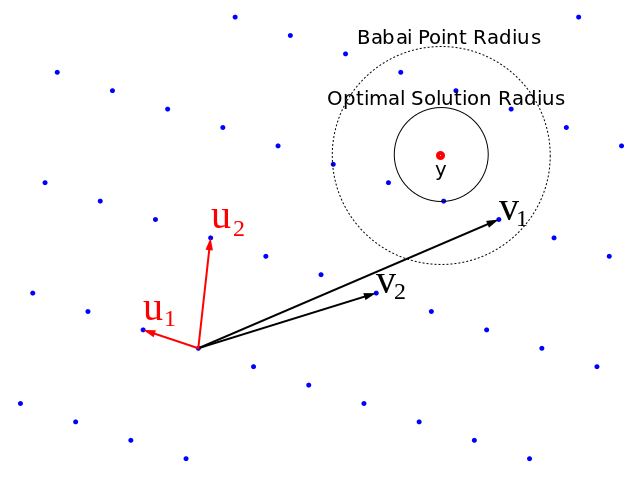
\includegraphics[scale=0.4]{latticebasis.png}
\caption{An example of a lattice with two different sets of basis vectors.}
\label{fig:latticeBasis}
\end{figure}

In this context, the ILS and BILS problems can be thought of as a search for the closest lattice point to some real point $y$. This thesis will not focus on the geometrical lattice interpretation of the problem; for more details on it, see \cite{AgrEVZ02}.

\vsp \section{Applications}

Some important applications such as MIMO wireless signal decoding depend on the
solution of the BILS problem. MIMO stands for ``multiple-input
multiple-output'', it refers to the case where a wireless system has multiple
input antennas transmitting a signal which is received by multiple output
antennas. The purpose of a MIMO system is to maximize the throughput of the communications channel. Throughput is defined as ''the average rate of successful message delivery over a communication channel``. 

The signal received is our input vector $y$ from
\eqref{eq:realLSModel}, it has undergone some linear transformation by the known
``channel matrix'' $H$ (design matrix) and some noise has been introduced during
the transmission. Originally, we know that each element of $x$ came from some
finite set of symbols that we may want to transmit or receive (we model
this property with $\boxcon$). The purpose of such a system is to maximize
throughput, however, the overall throughput of the system will depend on how
quickly and accurately we can solve the BILS problem. Of course we need not solve the BILS
problem exactly each time, however under the assumption that the noise has $0$ mean and is
normally distributed, the BILS solution is more likely than any other possible
solution to be the true integer parameter vector $x$. For this reason, we say that a receiver which is decoding transmissions using an algorithm which solves the BILS problem exactly achieves ``optimal performance''; performance refers to the likelihood that the vector found by the decoder is equal to the transmitted vector $x$.

Another application of the ILS problem arises in global positioning systems where carrier phase measurements are used. In GPS, there are two types of measurements that can be used to determine the position of a receiver, code phase and carrier phase. Code phase measurements can give accuracy to a few meters, while carrier phase are accurate to centimeters. To make use of the more accurate carrier phase measurements, we must know how many cycles the carrier wave has gone through between the satellite and the receiver. The number of cycles will be an integer, we can form a linear model for this system and obtain an estimate at the number of cycles by solving an ILS problem. 

Other applications of BILS and ILS include cryptography and lattice design. For any application where the elements of $x$
are known to be integer, we should use ILS. If the elements of $x$ are drawn from some finite set, BILS is appropriate.

\vsp \section{Previous Work} \label{sec:prevWork}
Due to the important applications of the BILS and ILS problems, much work has gone into solving them efficiently. There have been many algorithms proposed that yield a fast, approximate solution to the problem, some giving statistical bounds on the likelihood of error. This thesis however will only deal with finding the optimal solution to the problem.  Even for finding the optimal solution to the ILS problem, there are a few completely different approaches. This thesis will further be restricted to considering only what are known as `enumeration based' approaches which are most often used in practice because of their efficiency and simplicity. The enumeration based approaches, as the name implies, try to find the optimal solution by enumerating vectors in the search space one element at a time until all possible solutions but one are eliminated. The order in which the elements of the solution vectors are enumerated plays a critical role in how long the search algorithm will take to run; the reasons for this will become clear later.

\vsp \subsection{Search Strategies}
In chapter \ref{chap:SESearch}, it will be shown that the enumeration process can be reduced to a tree search problem. The tree in question will have a depth of $n$; each node on a path from root to leaf represents a valid element in the solution vector. Therefore the tree will have exponential width. To see an example of such a tree, refer to figure \ref{fig:treeSearch}. The most widely used algorithm for the ILS search process, the Schnorr Euchner (SE) enumeration \cite{SchE94}, can be thought of as a fairly straight forward depth first search in such a tree. Other tree search algorithms may also be used to solve the problem with varying degrees of efficiency.

In the literature, some modifications to the best first tree search strategy have also been proposed to solve this problem. A few such proposals are given in \cite{MurGDC06}, \cite{XuWZW04}, \cite{FukMU04}, \cite{StuBF07} and \cite{DaiY08}. When doing a tree search, the disadvantage of the best first approach is that the memory requirements can be exponential in the worst case and there is a significant overhead to visit each tree node. Compared to the depth first search where the memory requirements are linear and there is very little cost to visit a node in the tree. The advantage of the best first approach is that it can guarantee to explore the least number of nodes in the tree. Some of the papers listed above propose a pure best first search, while others try to make some sort of trade off to achieve lower memory usage.

There have been some attempts to compare different enumeration algorithms for the ILS search process. One such paper is \cite{MurGDC06}. The authors here devise a common framework (based on a tree search) that many search algorithms can be described within and from there they can do a comparison on the estimated computational complexity of each. Unfortunately through this theoretical comparison, we can only relate the number of nodes in the search tree that will be explored by various algorithms, this does not consider the amount of time processing each node which is often a computational bottleneck.

There have been other suggestions to improve the enumeration based search algorithms as well. In \cite{StoVH08}, it is proposed that by using lower bounds on the residual from the optimal solution, we can shrink the search space (equivalently, prune the search tree). A few such lower bounds are given for special cases of the ILS problem and one for the general ILS and BILS problem. Unfortunately, the computational complexity of computing some of these bounds can be prohibitive since it adds to the processing that must be performed at each node in the tree. Overall it seems that these lower bounds do not offer a decrease in computational complexity during the search process if the search is performed on a reduced problem.

Another method that attempts to shrink the search space is given in \cite{SchFL09}. They propose a simple stopping criteria for the search process that in theory should allow it to terminate earlier. Unfortunately, the bound derived here is not tight enough to be useful in practice and is rarely or never satisfied. Also it is proposed that after computing the bound, one can increment it with a low risk of achieving a suboptimal solution; this thesis will not consider this since it is only concerned with the exact solution of the ILS and BILS problems. 

\vsp \subsection{Reduction Strategies}

As mentioned previously, the purpose of the ILS and BILS reduction is to transform the problem to an equivalent, but easier to solve one. This section will review some existing reduction strategies.

The standard reduction algorithm used in practice for the unconstrained ILS problems is the LLL reduction \cite{LenLL82}. It is an old but very effective reduction strategy. In \cite{Bor10}, it was found that many of the operations used in the original LLL algorithm are not always required as they do not affect the search process when the SE algorithm is used. The new reduction that results from applying only a subset of the operations is called the partial LLL reduction.

Unfortunately, neither the LLL reduction or partial LLL reduction are applicable to the BILS problem. For the BILS problem, there are other reduction strategies that focus only on permuting the columns of the matrix $H$, where the LLL reduction performs some other operations that will be described in \ref{chap:Reduction}. We can separate reduction algorithms which simply try and find some optimal permutation of the columns of the matrix $H$ into two categories, those that only use the information contained in the matrix $H$, and algorithms that use both the information in $H$ and the vector $y$.

Two algorithms that only use the information in $H$ are VBLAST \cite{FosGVW99} and SQRD \cite{WubBRKK01}. An examination of these two algorithms reveals very similar motivations behind each.

Algorithms that use the information in both $H$ and $y$ are a fairly new development. The first was \cite{SuW05} in 2005, and then \cite{ChaH05} in 2008. Numerical results show that these algorithms can offer great improvements over the previous reductions that use only the information contained in $H$.

\vsp \section{Objectives and Contribution}
With many different algorithms for both the reduction and search process, it is not always clear how they relate. In \cite{MurGDC06} the authors propose a tree search framework to compare various search algorithms. This is an interesting idea, but results from such a comparison may not relate to real applications run time since they do not consider the time spent at each step of each algorithm, only how many steps are taken to solve the problem. This thesis will consider combining two popular and efficient search strategies where a parameter will control the influence of each individual algorithm. Using actual run time simulation results from a comparison of this combined algorithm with various settings of its parameter, we can see the strengths of each of the different approaches. This allows us tune the new combined algorithm so that it outperforms either of the originals. This also provides some insight into the runtime performance comparison of each algorithm individually.

For the reduction step, the LLL reduction \cite{LenLL82} is the strategy most used in practice for the ILS problem. How the LLL reduction theoretically relates to the ILS problem has been studied in detail, and it also yields excellent results in practice. Unfortunately, for the BILS problem, the LLL reduction should not be used, the reason for this will be described in chapter \ref{chap:Reduction}. For the BILS problem, we are limited to performing only column permutations on the matrix $H$. There are a few algorithms which calculate how we should permute the columns of $H$, some of which were briefly described in section \ref{sec:prevWork}. Two more recent developments, \cite{ChaH05} and \cite{SuW05}, use both the matrix $H$ and the vector $y$ to calculate the permutations. These algorithms have shown excellent results. In this thesis it will be proven that these two algorithms are theoretically equivalent. Knowing that they are equivalent, we can use the best ideas from both to create a new reduction strategy that is faster than either of the originals and is numerically stable (the faster of the two original algorithms is not). Another advantage of these algorithms being equivalent is that since one had a geometric motivation and the other was derived algebraically, we now how both geometric and algebraic justification for why the column orderings given by these algorithms should help speed up the search process. Also, since the SW algorithm was derived through a geometric motivation and as such is described in terms of geometry in the original paper; this thesis will provide an algebraic explanation for the SW algorithm and offer some improvements to the original.

The motivation for the permutation based reduction strategies is not specific to the BILS problem; in theory these reduction strategies should reduce the run time for ILS problems as well. However, the very effective LLL reduction provides better results than using permutations alone. One way to think about what each type of algorithm is doing is, the LLL reduction finds a new set of shorter and more orthogonal basis vectors, while the permutation based reductions are just finding an ordering for these vectors that performs well in the search process. Consider figure \ref{fig:latticeBasis} suppose the original matrix $H$ has columns $v_1$ and $v_2$, the LLL reduced matrix may have columns $u_1$ and $u_2$. It is known that shorter more orthogonal basis vectors are preferable in the search process. By first performing LLL reduction to get a good set of basis vectors, and then applying a permutation based reduction to re-order them, we can sometimes greatly improve the performance of the search process. In this thesis, the strategy of first applying a LLL reduction, and then column permutations will be explored.

\vsp \section{Outline}
The rest of the thesis will be organized as follows;

In chapter \ref{chap:SESearch}, the Schnorr-Euchner (SE) enumeration algorithm \cite{SchE94} will be presented in detail, much of the remainder of the thesis will use ideas and notation which comes from this algorithm. Also, since the reduction processes are trying to optimize the search process, it is critical to first understand the search process before considering the reduction.

In chapter \ref{chap:Reduction}, an explanation will be given for why we need different reduction strategies for BILS and ILS problems. Then, strategies for reducing BILS and ILS problems will be presented separately. A new BILS reduction strategy will be introduced. Also it will be explained how we can take advantage of the BILS reduction for ILS many problems.

In chapter \ref{chap:Searches}, some other notable search algorithms and modifications to the basic SE enumeration will be given. Also, a new hybrid search algorithm is proposed which combines two of the basic algorithms in order to take advantage of the positive features of each.

Finally, chapter \ref{chap:Conclusion} will give a summary and highlight areas where some future work could be done.

\chapter{Schnorr-Euchner Enumeration} \label{chap:SESearch}

There are many search algorithms that have been proposed to solve the unconstrained ILS problem. One of the most effective algorithms in terms of both overall runtime and memory consumption is the Schnorr-Euchner enumeration \cite{SchE94}. In this section, the SE algorithm will be presented in detail, since concepts from it will be used throughout the remainder of the thesis.

Let $H$ have the QR factorization
$$
H=[Q_1, Q_2] \bmx R \\ 0 \emx,
$$
where $[\underset{n}{Q_1}, \underset{m-n}{Q_2}]  \in \mathbb{R}^{m\times m}$ is orthogonal
and $R\in \mathbb{R}^{n\times n}$ is upper triangular. 
Then, with $\bar{y}=Q_1^Ty$ the ILS problem \eqref{eq:ils0} is reduced to 
\be 
\label{eq:ils}
\min_{x \in  {\mathbb{Z}}}  \| \by- Rx \|_2.
\ee

We would like to enumerate as few elements as possible, $x \in \mathbb{Z}^n$ while still guaranteeing the optimal solution. Suppose we start with some initial bound on the error,
\be 
\label{eq:searchIneq0}
\min_{x \in  {\mathbb{Z}}}  \| \by- Rx \|_2 \le \beta. 
\ee
We will discuss some better ideas for choosing an initial $\beta$ in later chapters, however one simple method is as follows, let $b$ be the real LS solution and $\lfloor b \rceil$ is $b$ with each element rounded to the nearest integer, and then calculate the residual $\left \| R \lceil b \rfloor - \bar{y} \right \|_2^2$. We may use this residual as the initial $\beta$ since the optimal solution must have a residual less than or equal to it. The inequality \eqref{eq:searchIneq0} defines an ellipsoid in terms of $x$ or a hyper-sphere in terms of the lattice points $w=Rx$ with radius $\beta$. For this reason, the problem is sometimes referred to as ``Sphere Decoding''.

Define
\begin{equation}
 c_k = (\bar{y}_k - \sum_{j=k+1}^nr_{kj}x_j)/r_{kk}, \; k=n, n-1,\ldots, 1,
\label{eq:searchC}
\end{equation}
where when $k=n$ the sum in the right hand side does not exist.
Then \eqref{eq:searchIneq0} can be rewritten as
\begin{equation}\label{eq:searchIneq1}
\min_{x \in  {\mathbb{Z}}} \sum_{k=1}^n r_{kk}^2(x_k-c_k)^2 \le \beta,
\end{equation}
which implies the following
set of inequalities:
\begin{align}
&\text{level } k: \ \ r_{kk}^2(x_k-c_k)^2 < \beta -\sum_{i=k+1}^nr_{ii}^2(x_i-c_i)^2, \label{eq:searchLevelK}
\end{align}

Defined for $k=n,n-1,\ldots, 1$. Observing equation \eqref{eq:searchLevelK} we see that the values for $x_k$ which will satisfy the inequality depend only on which values were chosen for $x_{k+1:n}$. The SE search process will now be described.

We begin the search process
at level $n$, therefore the valid values for $x_n$ only depends on the initial $\beta$. Choose $x_n = \lfloor c_n \rceil$, the nearest integer to $c_n$. If the inequality \eqref{eq:searchLevelK} with $k=n$
is not satisfied, it will not be satisfied for any integer, this means $\beta$
was chosen to be too small, it must be enlarged and the search restarted. With $x_n$ fixed, we can move
to level $n-1$ and choose $x_{n-1} = \lfloor c_{n-1} \rceil$ with $c_{n-1}$ calculated as in \eqref{eq:searchC}. At this point it is possible that the inequality \eqref{eq:searchLevelK} is no longer satisfied. If this is the case, we must move back to level $n$ and choose $x_n$ to be the second nearest integer to $c_n$.  We will continue this procedure until we reach
level 1, moving back a level if ever the inequality for the current level is no longer satisfied. When we reach level $1$, we will have found an integer point $\hat{x}$. Since $\hat{x}$ satisfies \ref{eq:searchIneq1}, we can use it to define a new, smaller radius which will effectively shrink the search space since there will be fewer valid choices for values of $x$.  To do this, update $\beta = \left \| \bar{y} - R\hat{x} \right \|_2^2$ and try to find a better integer point which lies in the new, smaller ellipsoid. We do this by continuing the search process from the current level after the radius has been tightened. The next step in the process will be to move back to level $2$ since no new choice for $x_1$ will give a better solution. Finally in the search process, when we can no longer find any $x_n$ to satisfy \eqref{eq:searchLevelK} with $k=n$, the search process is complete and the last integer point $\hat{x}$ found is the solution. If we initially set $\beta = \infty$ the first point $\hat{x}$ that we find is known as the Babai point.

\begin{figure}
\centering
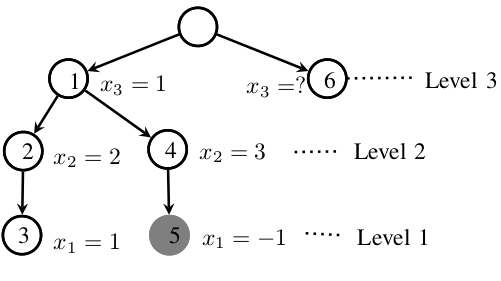
\includegraphics{searchtree.png}
\caption{An example of the search process with solution $x = [-1,3,1]^T$.}
\label{fig:treeSearch}
\end{figure}

The above search process is actually a depth-first tree search in a tree of height $n$, see Fig.\ \ref{fig:treeSearch},
where the number  in a node  denotes the step number at which the node is encountered. Each edge going from level $i$ to $i-1$ represents fixing $x_{i-1}$ to some value, and each edge will have a weight which is given by $r_{ii}^2(z_i -
c_i)^2$. Notice that if we take the sum of these weights from $m..i$ we simply get the partial
residual for fixing $x_{i:m}$, which is defined as $\left \| R_{i:m,i:m}x_{i:m} -
\bar{y}_{i:m} \right \|_2^2$. This implies that each leaf in the tree
represents an integer vector $x \in \mathbb{R}^m$ and its weight is the residual $\left \|
Rx - \bar{y} \right \|_2^2$. This means that the ILS problem is equivalent to
finding the lowest-weight leaf in the tree. The SE enumeration takes advantage
of the fact that we can easily calculate the lowest cost child of any given
node to make the depth first search more efficient. Compared to a standard tree search problem where to find the lowest cost edge leaving a given node you may have to check each edge individually. In fact we can easily visit
the children of a node in order of increasing weight or cost, that is what we are doing when we initially choose $x_k = \lfloor c_k \rceil$, and next choose it to be the second and third nearest integer to $c_k$.

A modification of the SE enumeration can be used to solve the BILS problem. To ensure that we remain within the box constraint, instead of choosing $x_k = \lfloor c_k \rceil$ at step $k$, we choose $x_{k} = \lfloor c_{k} \rceil_{{\cal B}_{k}}$, where ${\cal B}_{k}$ comes from \eqref{eq:boxCon}. Suppose $x_{k-1}:x_n$ are fixed, then we must also ensure that as we explore the node corresponding to the second nearest integer (and all subsequent integers) for $x_k$ that we remain within the box constraint. This is trivial to accomplish, we simply stop incrementing $x_k$ if we hit the upper bound, and stop decrementing it if we hit the lower bound. If all values for $x_k$ that are within the box constraint have been used up but we are still within the area defined by the ellipsoid, we move back to level $k-1$. Following this process will yield the optimal BILS solution. For more information on the BILS implementation of the SE algorithm, see \cite{ChaH05}.

\chapter{Reduction Strategies} \label{chap:Reduction}

Consider the ILS problem \eqref{eq:ils0}. The goal of the reduction is to modify the matrix $H$ in such a way that we still obtain the same solution $x$, but in fewer steps. With this goal, it is essential to know what types of operations we are allowed to perform on the matrix $H$ so that the solution $x$ is not modified. The first type of operation to consider is the orthogonal transformation. Suppose we apply some orthogonal matrix $Q$ from the left, then it is easy to see that \eqref{eq:ils0} becomes: 
\begin{align}
&\min_{x\in {\mathbb{Z} }}  \| QHx - y \|_2\\
=&\min_{x\in {\mathbb{Z} }}  \| Q^T(QHx - y) \|_2\\
=&\min_{x\in {\mathbb{Z} }}  \| Hx - \bar{y} \|_2
\end{align}

The second type of transformation that we may apply to the matrix $H$ is any unimodular matrix. Unimodular matrices are square, integer matrices with determinant $+/-1$. Let $Z$ be some unimodular matrix. Another property of unimodular matrices is that the equation $Zx=b$ always has an integer solution $x$ if $b$ is integer, this is because the inverse of the unimodular matrix is also guaranteed to be integer and unimodular. This property is very useful for our application. Consider applying such a unimodular matrix $Z$ to $H$ from the right, \eqref{eq:ils0} becomes: 
\begin{align}
&\min_{x\in {\mathbb{Z} }}  \| HZx - y \|_2\\
=&\min_{\hat{x}\in {\mathbb{Z} }}  \| H\hat{x} - y \|_2\\
\end{align}
When we solve this new ILS problem, we will obtain some solution $\hat{x}$. If $Z$ is a known unimodular matrix, we can solve the system $Zx = \hat{x}$ to find $x$, the ILS solution to the original problem. Note that if Z were not unimodular, we would have no guarantee that the solution $x$ would be integer.

Finally, it is worth mentioning that we may apply permutation matrices to $H$ as well, although they are just a special case of unimodular matrices. It is obvious that the effect on the solution from applying a permutation matrix is only to re-order the elements of the solution vector $x$.

When reducing the BILS problem we must be more careful. Consider the constraints on the solution $x$, \eqref{eq:boxCon}. Applying orthogonal matrices to $H$ from the left has no effect on $x$, so the constraints are also unaffected. Applying permutation matrices to H from the right will re-order the elements of the solution $x$, so we must re-order the elements in the constraint vectors as well, which is a trivial operation. However if we apply a general unimodular matrix $Z$ to $H$ from the right, we can no longer easily enforce the constraints on the solution, the simple box constraints become complicated. To see why this is the case, recall the SE search process. Suppose the search is currently at some level $k$ and we would like to know to which value we should fix $\hat{x}_{k-1}$ (note that $\hat{x}$ denotes $Zx$). We know that $l_{k-1} \le x_{k-1} \le u_{k-1}$, but to determine such a bound for $\hat{x}_{k-1}$, we would need to know the entire vector $\hat{x}$ in order to compute $Z^{-1}_{k-1,:}\hat{x}$. At this point in the search, we only know the last $k$ elements of it. The only way to complete the search process is to ignore the bounds on $\hat{x}$, find a potential solution, compute $x = Z^{-1}\hat{x}$, and then check if each element of $x$ is within the bounds. This is extremely inefficient since many potential solutions could be eliminated very early on in the search if we were able to enforce the constraints during the search process. It is for this reason that when reducing BILS problems, we only consider orthogonal transformations and column permutations.

\vsp \section{BILS Reduction Algorithms} \label{sec:BILSReduction}

Due to the difficulty of applying general unimodular matrices to reduce the BILS problem, the algorithms in this section will focus on finding some permutation of the columns of the matrix $H$ in order to optimize the search process.

\vsp \subsection{Previous Reductions}
The V-BLAST algorithm \cite{FosGVW99} mentioned in \ref{sec:prevWork} is a commonly used strategy to calculate the column permutations for $H$. Suppose we are working with $R$, which comes from the QR factorization of $H$. Recall that the product of the diagonal elements of an upper triangular matrix is equal to the matrices determinant, and this value is invariant under permutation. This means that any time we swap two columns in the matrix $H$ and re-calculate the QR factorization, one diagonal element of $R$ will always increase and the other will decrease.

The goal of the V-BLAST algorithm is to proceed from $k=n \dots 1$ and find the column $h_p$ from the set of columns $h_1 \dots h_k$ such that when $h_p$ and $h_k$ are swapped, the diagonal element $r_{kk}$ is maximal There are efficient algorithms to compute such a column ordering, one such algorithm will become obvious later in this section.

In \cite{ChaH05}, the SQRD column reordering strategy originally presented in \cite{WubBRKK01} for the same purpose as V-BLAST, was proposed for this purpose. In the SQRD algorithm, we perform the QR decomposition from columns $k = 1 \dots n$, at each step choosing as the $k^{th}$ column the column from the set $k \dots n$ which gives the smallest diagonal element $r_{kk}$. This should yield large $r_{kk}$ toward the end of the matrix since the product of the diagonal elements is a constant. Note that both SQRD and V-BLAST only use the information in the matrix $H$.

In \cite{SuW05}, Su and Wassell considered the geometry of the BILS
problem for the case that $H$ is nonsingular and proposed a new column reordering algorithm (to be called
the SW algorithm from here on for convenience) which uses all information of the BILS problem.
Unfortunately, the geometric interpretation of this algorithm is hard to understand.
Probably due to page limit, the description of the algorithm is very concise, 
making efficient implementation difficult for ordinary users.

This thesis will give some new insight of the SW algorithm from an algebraic point of view.
Some modifications will be made so that the algorithm becomes more efficient
and easier to understand and furthermore it can handle a general full column rank $H$.
It is worth mentioning that the SW algorithm is not numerically stable. The numerical stability is not
necessarily crucial since a wrong answer just results in a different set of
permutations for the columns of H where any set of permutations is allowable.
Until this point, other column reordering algorithms only considered the matrix $H$.

Independently  Chang and Han in \cite{ChaH05} proposed
another column reordering algorithm (which will be referred to as  CH).
Their algorithm also uses all information of the BILS problem and the derivation
is based on an algebraic point of view. It is  easy to see from the equations in
the search process exactly what the CH column reordering is doing and why we
should expect a reduced complexity in the search process. The detailed
description of the CH column reordering is given in \cite{ChaH05} and it is easy
for others to implement the algorithm.
But our numerical tests and theoretical analysis indicated CH has a higher complexity than SW, when SW
is implemented efficiently.
Our numerical tests also showed that CH and SW {\em almost} always   
produced the same permutation matrix $P$, the only exception is when then matrix $H$ is very ill conditioned.

In this section it will be shown that the CH algorithm and the  (modified)  SW algorithm give the same
column reordering in theory. This is interesting because both algorithms were derived through different motivations
and we now have both a geometric justification and an algebraic justification 
for why the column reordering strategy should reduce the complexity of the search.
Furthermore, using the knowledge that certain steps in each algorithm are equivalent,
we can combine the best parts from each into a new algorithm. The new algorithm
has a lower flop count than either of the originals.
This is important to the successive interference cancellation decoder, 
which computes a suboptimal solution to the BILS problem. When computing suboptimal solutions, the overall runtime may not be so dominated by the search, and the complexity of the reduction becomes a bottleneck.
The new algorithm can be interpreted in the same way as CH,
so it is easy to understand. 

In the following subsections, the CH and SW algorithms will be described in detail. This is necessary to understanding the proof of their equivalence and to see the motivation for the new algorithm. Also, a new algebraic interpretation and some improvements will be given for the SW algorithm. Finally the proof of equivalence of CH and SW will be given, and the new algorithm will be presented.

\vsp \subsection{CH Algorithm} \label{subsec:CH}
The CH algorithm first computes the QR factorization of $H$,
then  tries to reorder the columns of $R$.
The motivation for this algorithm comes from observing equation \eqref{eq:searchLevelK}.
If the inequality is false we know that the current choice for the value of
$x_k$ given $x_{k+1:n}$ are fixed is incorrect and we prune the search tree (we do not need to explore the subtree for the current node). We
would like to choose the column permutations so that it is likely that the
inequality will be false at higher levels in the search tree, this way we waste less time exploring solutions that are not optimal. The CH column reordering strategy
does this by trying to maximize the left hand side of  \eqref{eq:searchLevelK} with large values of $\left | r_{kk}
\right |$ and minimize the right hand side by making $\left | r_{kk}(x_k-c_k) \right |$
large for values of $k = n,n-1, \dots, 1$.

Here we describe  step 1 of the CH algorithm, which determines the last column of the final $R$ 
(or equivalently the last column of the final $H$).
Subsequent steps are the same but are applied to a subproblem that is one dimension smaller. 
In step 1, for $i = 1,\dots,n$ we interchange
columns $i$ and $n$ of  $R$ (thus entries of $i$ and $n$ in $x$ are also swapped), then return $R$ to upper-triangular
by a series of Givens rotations applied to $R$ from the left, which  are also applied to $\bar{y}$. The following example demonstrates the process of returning the matrix $R$ to upper triangular after column $n$ is swapped with column $2$ in a $5 \times 5$ matrix.

\begin{equation} \label{eq:swappedCols}
\begin{bmatrix}
x & x & x & x & x\\ 
  & x & x & x & x\\ 
  & x & x & x &  \\ 
  & x &  &  x &  \\ 
  & x &  &    & 
\end{bmatrix}
\end{equation}

Equation \ref{eq:swappedCols} shows the matrix directly after the column swap. We want to restore it to upper triangular. To do so, we start by using $n-i$ Givens rotations to zero the subdiagonal elements in column $i$, in this case $i = 2$. Each Givens rotation is an orthogonal matrix which adds multiples of two rows to eachother, for our purposes, we would like to add only multiples of adjacent rows. A Givens rotation that uses row $k$ to zero element $j$ in row $k+1$ is defined in equation \eqref{eq:givensRotation}, denote such a Givens rotation as $G_{k,k+1}$:

\begin{equation} \label{eq:givensRotation}
\begin{bmatrix}
I_{k-1} &  &  & \\ 
 & c & -s & \\ 
 & -s & c & \\ 
 &  &  & I_{n-k-1}
\end{bmatrix} ,\quad c^2+s^2=1
\end{equation}
Where $c=\frac{R_{k,j}}{\sqrt{R_{k,j}^2+R_{k+1,j}^2}}$ and $s=\frac{R_{k+1,j}}{\sqrt{R_{k,j}^2+R_{k+1,j}^2}}$.

We can use rotations $G_{n-1,n}, G_{n-2,n-1} \dots G_{i,i+1}$ to zero the subdiagonal elements in the $i^{th}$ column, however this will create subdiagonal elements in columns $i+1 \dots n$. Equation \eqref{eq:subDiagEntries} shows the matrix after applying this first round of Givens rotatations.

\begin{equation} \label{eq:subDiagEntries}
\begin{bmatrix}
x & x & x & x & x \\ 
  & x & x & x & x \\ 
  &   & x & x & x \\ 
  &   & x & x &   \\ 
  &   &  &  x & 
\end{bmatrix}
\end{equation}

We can now use a second round of Givens rotation to eliminate the new subdiagonal entries and restore the matrix to upper triangular. We use the rotations in the following order, $G_{i+1,i+2}, G_{i+2,i+3} \dots G_{n-1,n}$ where each rotation should zero the subdiagonal element in the corresponding column.

To avoid confusion, we denote the new $R$ after restoring the upper triangular structure by $\hat{R}$ and the new $\bar{y}$ by $\hat{y}$.
We then compute  $c_n=\hat{y}_n/\hat{r}_{n,n}$ and 
\be
x_i^c=\arg\min_{x_i\in {\cal B}_i}\left |\hat{r}_{nn}(x_i- c_n) \right | = \left \lfloor c_n \right \rceil_{{\cal B}_i},
\label{eq:xic}
\ee
where the superscript $c$ denotes the CH algorithm. 
Let $\bar{x}_i^c$ be the second closest integer in ${{\cal B}_i}$ to $c_n$,
i.e.,  
$\bar{x}_i^c= \left \lfloor c_n \right \rceil_{{\cal B}_i\backslash x_i^c}.$
%So $\bar{x}_i^c = x_i^c \pm 1$.
Define
\be
\dist_i^c = |\hat{r}_{nn}( \bar{x}_i^c -c_n) |, 
\label{eq:dic}
\ee
which represents the partial residual given when $x_i$ is taken to be $\bar{x}_i^c$.
Let $j = {\arg\max}_i \dist_i^c$.
Then  column $j$ of the original $R$ is chosen to be the $n^{th}$ column of the final $R$.
%The algorithm then applies the Givens rotations that were used to restore $R$ to
%upper triangular to $\bar{y}$ and 
With the corresponding updated upper triangular $R$ and $\bar{y}$
(here for convenience we have removed hats),
the algorithm then updates  $\bar{y}_{1:n-1}$ again
by setting $\bar{y}_{1:n-1}: = \bar{y}_{1:n-1} - r_{1:n-1,n}x_j$ where $x_j=x_j^c$. 
%Note that we use $z$ to denote the permuted $x$.
Choosing  $x_j$ to be  $x_j^c$ here is exactly the same as what the search process does.
We then continue to work on the subproblem 
\be
\min_{\tilde{x}\in \mathbb{Z}^{n-1}} \left \| \bar{y}_{1:n-1}-R_{1:n-1,1:n-1}\tilde{x} \right \|_2,
\label{eq:subc}
\ee
where $\tilde{x}=[x_1,\ldots, x_{j-1}, x_n, x_{j+1}, \ldots x_{n-1}]^T$ satisfies the corresponding box constraint.
The pseudocode of the CH algorithm is given in Algorithm \ref{alg:CH}.

To determine the last column, CH finds the permutation to 
maximize $\left |r_{nn}(\bar{x}_i^c-c_n) \right |$. Using $\bar{x}_i^c$ instead of $x_i^c$
ensures that $\left | \bar{x}_i^c-c_n \right |$ is never less than $0.5$ but
also not very large. This means that usually if $\left | r_{nn}(\bar{x}_i^c-c_n)
\right |$ is large, $\left | r_{nn} \right |$ is large as well and the
requirement to have large $|r_{nn}|$ %in order from $m,\dots,1$  
is met.
Using $x_i^c$ would not be a good choice because $\left | x_i^c - c_n \right |$ might be 
very small or even $0$, then column $i$ would not be chosen to be column $n$
even if the corresponding $|r_{nn}|$ is large and on the contrary a column with small $|r_{nn}|$
but large $|x_i^c-c_n|$ may be chosen.

Now we will consider the complexity of CH. The 
significant cost comes from line \ref{l:chg} in Algorithm \ref{alg:CH},
which requires $6(k-i)^2$ flops.
If we sum this cost over all loop iterations and add the cost of the QR factorization by Householder transformations, 
we  get a total complexity of $0.5n^4+2mn^2$ flops.

\begin{algorithm}
\caption{CH Algorithm - Returns $p$, the column permutation vector}
\label{alg:CH}
\begin{algorithmic}[1]
\STATE $p := 1:n$
\STATE $p' := 1:n$
\STATE Compute the QR factorization of $H$: $\bsmx Q_1^T \\ Q_2^T \esmx H= \bsmx R\\ 0 \esmx$
             and compute  $\bar{y} : = Q_1^Ty$
  \FOR{$k=n$ to $2$}
  	\STATE $maxDist := -1$
    \FOR{$i=1$ to $k$}
    	\STATE $\hat{y} := \bar{y}_{1:k}$
    	\STATE $\hat{R} := R_{1:k,1:k}$
        \STATE  \label{l:chg} swap columns $i$ and $k$ of $\hat{R}$, return it  to upper
triangular with Givens rotations, also apply the Givens rotations to $\hat{y}$ %\hfill ($6(k-j)^2$ flops)  
        \STATE $x_i^c := \left \lfloor\hat{y}_k/\hat{r}_{k,k}\right
\rceil_{{\cal B}_i}$
        \STATE $\bar{x}_i^c := \left \lfloor\hat{y}_k/\hat{r}_{k,k}\right
\rceil_{{\cal B}_i\backslash x_i^c}$
        \STATE $dist_i^c := \left | \hat{r}_{k,k}\bar{x}_i^c - \hat{y}_k
\right | $
        \IF{$dist_i^c > maxDist$}
        	\STATE $maxDist := dist_i^c$
        	\STATE $j := i$
        	\STATE $R' := \hat{R}$
        	\STATE $y' := \hat{y}$
        \ENDIF
    \ENDFOR
    \STATE $p_k := p'_j$
    \STATE Interchange the intervals ${{\cal B}_k}$ and ${{\cal B}_{j}}$
    \STATE Intechange entries $k$ and $j$ in $p'$
    \STATE $R_{1:k,1:k} := R'$
    \STATE $\bar{y}_{1:k} := y' - R'_{1:k,k}x_j^c$
  \ENDFOR
  \STATE $p_1 := p'_1$
\end{algorithmic}
\end{algorithm}

\vsp \subsection{SW Original Algorithm} \label{subsec:SW}
The motivation for the SW algorithm comes from examining the geometry of the search process.

\ifx\du\undefined
  \newlength{\du}
\fi
\begin{figure}
\centering
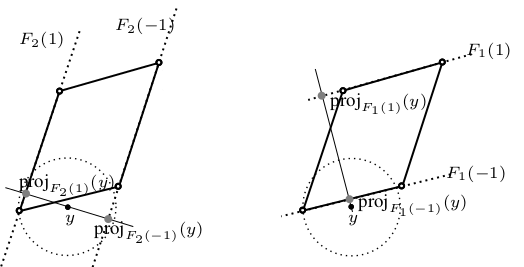
\includegraphics{sumotivation.png}
\caption{Geometry of the search  with two different column ordering.}
\label{SEGeometry}
\end{figure}

Fig.\ \ref{SEGeometry} shows a 2-D BILS problem;
\ref{SEGeometry}(a) represents the original column ordering and 
\ref{SEGeometry}(b) is after the columns have been swapped.

In the SW algorithm $H=[h_1,\ldots, h_n]$ is assumed to be square and non-singular.
Let 
$$
G =[g_1,\ldots, g_n]= H^{-T}.
$$ 
For any  integer $\alpha$,   \cite{SuW05} defines the
affine sets, $F_i(\alpha) = \{w \ | \ g_i^T(w-h_i\alpha) = 0\}$.
%which can also be thought of as $h_i$ shifted by the integer $\alpha$.
The lattice points generated by $H$ occur at the intersections of these affine sets. 
Let the orthogonal projection of a vector $s$ onto a vector $t$ be denoted as
$\mbox{proj}_t(s)$, then %\cite{SuW05} claims that 
the orthogonal projection of some vector $s$ onto $F_i(\alpha)$ is 
$\mbox{proj}_{F_i(\alpha)}(s) = s -\mbox{proj}_{g_i}(s-h_i\alpha).$ 
Therefore the orthogonal distance between $s$ and
$F_i(\alpha)$ is $\dist(s,F_i(\alpha)) =  \| s - \mbox{proj}_{F_i(\alpha)}(s) \|_2$. 
%%%%%%%%%%%%
%\footnote{XW: Why don't they simply say the distance is just $\|\mbox{proj}_{g_i}(s-h_i\alpha)\|$?
%It's quite weird. SB: I'm not sure, it seems like that projection is equivalent
%and much simpler and we could avoid using the affine sets $F_i(s)$}
%%%%%%%%%%%%%%%%
In \cite{SuW05}, the points labeled $\mbox{proj}_{F_2(1)}(y)$ and
$\mbox{proj}_{F_2(-1)}(y)$ in Fig.\  \ref{SEGeometry}
are called residual targets  and ``represent the
components [of $y$] that remain after an orthogonal part has been projected
away.''  

Note that $F_2(\alpha)$ in Fig.\ \ref{SEGeometry} is a sublattice of dimension $1$.  
Algebraically it is the lattice generated by $H$ with column
$2$ removed. It can also be thought of as a subtree of the search tree where
$x_2 = \alpha$ has been fixed. 
In the first step of the search process for a general case,   $x_n$ is chosen to be
 $x_n=\arg\min_{\alpha\in {\cal B}_n}\dist(y,F_n(\alpha))$; thus $F_n(x_n)$ is the nearest affine set to $y$. 
Actually the value of $x_n$ is identical to $\lfloor c_n \rceil_{{\cal B}_n}$ given in Chapter ~\ref{chap:SESearch},
which will be proven later.
Then   $y$ is updated  as $y := \mbox{proj}_{F_n(x_n)}(y) - h_nx_n$. If we look
at Fig.\ \ref{SEGeometry}, we see that the projection $\mbox{proj}_{F_n(x_n)}(y)$ moves $y$ onto $F_n(x_n)$, while the subtraction of $h_nx_n$ algebraically fixes the value of $x_n$. This is necessary because in subsequent steps we will not consider the column $h_n$.

We now apply the same process to the new $n-1$ dimensional search space
$F_n(x_n)$. If at some level $i$, $\min_{\alpha\in {\cal B}_i}\dist(y,F_i(\alpha))$ exceeds the current
search radius, we must move back to level $i+1$. % and choose $x_i = x_i \pm 1$.
When the search process reaches level $1$ and fixes $x_1$, it updates the radius to  
$\dist(y,F_1(x_1))$ and moves back up to level $2$.

Note that this search process is mathematically equivalent to the one described in Chapter
\ref{chap:SESearch}; the difference is that it  does projections
because  the generator matrix is not assumed to be upper-triangular. 
Computationally the former is more expensive than the latter since the cost for QR factorization is only incurred once and we avoid the expensive projections.

To see the motivation of the SW algorithm for choosing a particular column ordering,
consider Fig.\ \ref{SEGeometry}. Suppose the search algorithm has knowledge of
the residual for the optimal solution (the radius of the circle in the diagram).
With the column ordering chosen in (a), there are two possible choices for $x_2$,
leading to the two dashed lines $F_2(-1)$ and $F_2(1)$ which cross the circle. This means
that we will need to compute $x_1$ for both of these choices
before we can determine which one leads to the optimum solution. In (b), there
is only one possible choice for $x_1$,  leading to the only dashed line $F_1(-1)$
which crosses the circle, meaning we only need to find $x_2$ to find the optimum solution.
Since the projection resulting from the correct choice of $x_2$ will always be
within the sphere, it makes sense to choose the ordering which maximizes the
distance to the second best choice for $x_2$ in hopes that the second nearest
choice will result in a value for $\min_{\alpha\in {\cal B}_2}\dist(y,F_2(\alpha))$ outside the sphere and the
dimensionality can be reduced by one. 
For more detail on the geometry, see  \cite{SuW05}.

The following will give an overview of the SW algorithm as given in
\cite{SuW05} but described in a framework similar to what was used to describe
CH. In the first step to determine the last column, for each $i = 1, \dots, n$,
we compute 
\be
x_i^s \!=\! \arg\min_{\alpha\in {\cal B}_i}\dist(y,F_i(\alpha)) 
\!=\!  \arg\min _{\alpha\in {\cal B}_i}| y^Tg_i - \alpha | \!=\! \left \lfloor y^Tg_i \right \rceil_{{\cal B}_i},
\label{eq:xis}
\ee
where the superscript $s$  stands for the SW algorithm.
Let $\bar{x}_i^s$ be the second closest integer in ${{\cal B}_i }$ to $y^Tg_i$, i.e.,
$\bar{x}_i^s = \left \lfloor y^Tg_i \right \rceil_{{\cal B}_i\backslash x_i^s}.$
Let $j = \arg\max_i  \dist (y,F_i(\bar{x}_i^s))$. 
Then SW chooses column $j$ as the last column of the final reordered $H$,
 updates $y$ by setting 
$y:=\mbox{proj}_{F_j(x_j^s)}(y) -h_jx_j^s$  and 
updates $G$ by setting $ g_i: = \mbox{proj}_{F_j(0)}(g_i)$ for all $i\neq j$. 
After $G$ and $y$ have been updated, the algorithm continues to find column $n-1$ in the
same way etc. The pseudo-code of the SW algorithm is given in Algorithm \ref{alg:SWOrig}.
\begin{algorithm}
\caption{SW Algorithm - Returns $p$, the column permutation vector}
\label{alg:SWOrig}
\begin{algorithmic}[1]
\STATE $p := 1:n$
\STATE $p' := \{1, 2, \ldots, n\}$
\STATE \label{l:swG} $G := H^{-T}$ \hfill %($2n^3$ flops)
\FOR{$k=n$ to $2$}
	\STATE $maxDist := -1$
	\FOR{$i \in p'$}
		\STATE $x_i^s := \left \lfloor  y^Tg_i \right \rceil_{{\cal B }_i}$ \hfill% ($2n$ flops)
		     \label{l:swx}
		\STATE $\bar{x}_i^s := \left \lfloor y^Tg_i \right \rceil_{{{\cal B }_i}{\backslash x_i^s}}$
		    \label{l:swbx}
		\STATE  \label{l:swd} $\dist_i^s := \dist(y,F_i(\bar{x}_i^s))$ %\hfill ($3n^2$ flops)
		\IF{$dist_i^s > maxDist$}
			\STATE $maxDist := dist_i^s$
			\STATE $j := i$
		\ENDIF
	\ENDFOR
	\STATE $p_k := j$
	\STATE $p' := p' \backslash j$
	\STATE $y := \mbox{proj}_{F_j(x_j^s)}(y) -h_jx_j^s$  \label{l:swy}
	\FOR{$i \in p'$}
		\STATE \label{l:swg} $g_i := \mbox{proj}_{F_j(0)}(g_i) $ %\hfill ($2n^2$ flops) 
	\ENDFOR
\ENDFOR
\STATE $p_1 := p'$
\end{algorithmic}
\end{algorithm}

%Now we look at the complexity of Algorithm \ref{alg:SWOrig}.
Su and Wassell did not say how to implement the algorithm and did not give a complexity analysis.
The parts of the cost we must consider for implementation occur in
lines \ref{l:swd} and \ref{l:swg}.
Note that $ \dist(y,F_i(\bar{x}_i^s))=\|\mbox{proj}_{g_i}(y-h_i\bar{x}_i^s)\|_2$
and $\mbox{proj}_{F_j(0)}(g_i)= g_i -\mbox{proj}_{g_i} g_i$,
where $\mbox{proj}_{g_i}=g_ig_i^\dag = g_ig_i^T/\|g_i\|^2$. 
A naive implementation would first compute $\mbox{proj}_{g_i}$, requiring $n^2$ flops, then compute 
$\|\mbox{proj}_{g_i}(y-h_i\bar{x}_i^s)\|_2$ and $g_i -\mbox{proj}_{g_i} g_i$, each requiring $2n^2$ flops.
Summing these costs over all loop iterations we get a total complexity of $2.5n^4$ flops.
In the next subsection we will simplify some steps in Algorithm \ref{alg:SWOrig}
and show how to  implement them efficiently.

\vsp \subsection{SW Algorithm Interpretation and Improvements}
\label{sec:improvedSW}
In this section we give new algebraic interpretation of some steps in Algorithm 2,
simplify some key steps to improve the efficiency,
and  extend the algorithm to handle a more general case.
All line numbers refer to Algorithm \ref{alg:SWOrig}.

%At each step, we must compute  $x_i^s = \left \lfloor y^Tg_i \right \rceil_{{\cal B}_i }$ and $\dist_i^s$. 
First we show  how to efficiently compute $\dist_i^s$ in line \ref{l:swd}. 
Observing that $g_i^Th_i = 1$, we have
\begin{equation}
\label{eq:newDist}
\dist_i^s =   \|  g_ig_i^\dag (y-h_i\bar{x}_i^s)  \|_2 
=    | y^Tg_i -\bar{x}_i^s |/\| g_i  \|_2.
\end{equation} 
Note that $y^Tg_i$ and $\bar{x}_i^s$ have been computed in lines \ref{l:swx} and \ref{l:swbx}, respectively.
So the main cost of computing $\dist_i^s$ is the cost of computing $\|g_i\|_2$,
requiring only $2n$ flops. 
For $k=n$ in Algorithm 2,  $y^Tg_i=y^TH^{-T}e_i=(H^{-1}y)^Te_i$, i.e.,  $y^Tg_i$
is the $i^{th}$ entry of the real solution $x$ for $Hx=y$. 
The interpretation can be generalized to  a general $k$. 

In line \ref{l:swg} Algorithm 2,  
\begin{align}
g_i^{\small \mbox{new}} & \equiv \mbox{proj}_{F_j(0)}(g_i)   \nonumber \\
  & =(I- \mbox{proj}_{g_j})g_i=g_i- g_j(g_j^Tg_i/\|g_j\|_2^2). \label{eq:gup}
\end{align}
Using the last expression for computation needs only $4n$ flops
(note that $\|g_j\|_2$ has been computed before, see \eqref{eq:newDist}).
We can actually show that the above is performing updating of $G$, the Moore-Penrose generalized inverse of
$H$ after we remove its $j^{th}$ column. This will allow us to interpret the subsequent steps of SW as operating on a subproblem. For proof of this, see \cite{Cli64}.

In line \ref{l:swy} of Algorithm 2,
\begin{align}
y^{\small \mbox{new}} & \!\equiv\! \mbox{proj}_{F_j(x_j^s)}(y) - h_jx_j^s 
 \!=\! (y -  g_jg_j^\dag(y-h_jx_j^s)) - h_jx_j^s  \nonumber \\
   &=  (I-\mbox{proj}_{g_j})(y-h_jx_j^s). \label{eq:yup}  
\end{align}
This means that after $x_j$ is fixed to be $x_j^s$, $h_jx_j^s$ is combined with $y$ (the same
as CH does)  and then the vector is projected to the orthogonal complement of 
the space spanned by $g_j$. 
We can show that this guarantees that the updated $y$ is in the subspace spanned by
the columns of $H$ which have not yet been chosen.
This is consistent with the assumption that $H$ is nonsingular, which implies that 
the original $y$  is in the space spanned by  the columns of $H$.
However, it is not necessary to apply the orthogonal projector $I- \mbox{proj}_{g_j}$ to $y-h_jx_j^s$ in \eqref{eq:yup}.
The reason is as follows. 
In Algorithm 2, $y^{\small \mbox{new}}$ and $g_i^{\small \mbox{new}}$ will be used only for computing 
$(y^{\small \mbox{new}})^Tg_i^{\small \mbox{new}}$ (see line \ref{l:swx}).
But from \eqref{eq:gup} and \eqref{eq:yup}
\begin{align*}
(y^{\small \mbox{new}})^Tg_i^{\small \mbox{new}}
& =(y-h_jx_j^s)^T(I-\mbox{proj}_{g_j})(I-\mbox{proj}_{g_j})g_i \\
&=(y-h_jx_j^s)^Tg_i^{\small \mbox{new}}.
\end{align*}
Therefore, line \ref{l:swy} can be replaced by $y:=y-h_jx_j^s$.
This not only simplifies the computation but also is much easier to interpret---after $x_j$ is fixed to be $x_j^s$,  
$h_jx_j^s$ is combined into $y$ as in the CH algorithm.
Let $H_{:,1:n-1}$ denote $H$ after its $j^{th}$ column is removed. 
We then continue to work on the subproblem
\be
\min_{\check{x}\in \mathbb{Z}^{n-1}}\|y-H_{:,1:n-1}\check{x}\|_2, 
\label{eq:subs}
\ee
where $\check{x}=[x_1,\ldots,x_{j-1},x_{j+1},\ldots,x_n]^T$ 
satisfies the corresponding box constraint.
Here $H_{:,1:n-1}$ is not square. But there is no problem to handle
it, see the next paragraph.

In \cite{SuW05},  $H$ is assumed to be square and non-singular. 
In our opinion, this condition may cause confusion,
since for each $k$ except $k=n$ in Algorithm 2, 
the remaining columns of $H$ which have not been chosen do not form a square matrix.
Also the condition restricts the application of the algorithm to a general full column rank matrix $H$,
unless we transform $H$ to a nonsingular matrix $R$ by the QR factorization.
To extend the algorithm to a general full column rank matrix $H$, we need only 
replace line \ref{l:swG} by $G:=(H^{\dagger})^T$.
This extension has another benefit. 
We mentioned before that the updating of $G$ in line \ref{l:swg}
is actually the updating of the Moore-Pernrose generalized inverse 
of the matrix formed by the columns of $H$ which have not been chosen. 
So the extension makes all steps consistent.

To reliably compute $G$ for a general full column rank $H$,
we can compute the  QR factorization $H=Q_1R$ by the Householder transformations
and then solve the triangular system  $RG^T=Q_1^T$ to obtain $G$.
This requires $(5m-4n/3)n^2$ flops. 
Another less reliable but more efficient way to do this is to compute $G=H(H^TH)^{-1}$. 
To do this efficiently we would compute the Cholesky factorization  $H^TH = R^TR$ and solve 
$R^TRG^T = H^T$ for $G$ by using the triangular structure of $R$. 
The total cost for computing $G$ by this method can be shown to be $3mn^2+\frac{n^3}{3}$.
If $H$ is square and nonsingular, we would use the LU factorization with partial pivoting to compute $H^{-1}$
and the cost is $2n^3$ flops.

For the rest of the algorithm if we use the simplification and efficient implementations
mentioned above, we can show that it needs $4mn^2$ flops. 

We see the modified SW algorithm is much more efficient than both the CH algorithm
and the SW algorithm implemented in a naive way we mentioned in the previous subsection.

\vsp \subsection{Proof of Equivalence of SW and CH}
In this subsection we prove that  CH and  the modified  SW produce the same set of permutations
for a general full column rank $H$.
To prove this it will suffice to prove that $x_i^s = x_i^c$, $\bar{x}_i^s =\bar{x}_i^c$,
$\dist_i^s = \dist_i^c$ for $i=1, \ldots, n$ in the first step which determines the last column of the final reordered $H$
and that the subproblems produced for the second step of
each algorithm are equivalent. 

Proving $x_i^s = x_i^c$ is not difficult.
The only effect the interchange of columns $i$  and $n$ of $R$ in CH  
has on the real LS solution is that elements $i$ and $n$ of the solution are swapped.
Therefore $x_i^c$ is just the $i^{th}$ element of the real LS
solution rounded to the nearest integer in ${{\cal B}_i }$. 
Thus, with \eqref{eq:xic} and \eqref{eq:xis},
\be
x_i^c=   \lfloor (H^{\dagger}y)_i  \rceil_{{\cal B}_i }
=  \lfloor e_i^T H^{\dagger}y   \rceil_{{\cal B}_i }
=  \lfloor g_i^T  y \rceil_{{\cal B}_i } =x_i^s.
\label{eq:xics}
\ee
Therefore we also have $\bar{x}_i^c=\bar{x}_i^s$.

In CH, after applying a permutation $P$ to swap columns $i$ and $n$ of $R$,  
we apply $V^T$, a product of the Givens rotations, to bring $R$ back to a new upper triangular
matrix, denoted by $\hat{R}$, and also apply $V$ to $\bar{y}$, 
leading to  $\hat{y} = V^T\bar{y}$. 
Thus  $\hat{R}=V^T RP$ and $\hat{y} = V^T\bar{y}=V^TQ_1^Ty$. 
Then $H=Q_1R= Q_1V\hat{R}P^T$, $H^\dag= P\hat{R}^{-1}V^TQ_1^T$, 
$g_i=(H^\dag)^Te_i=Q_1V\hat{R}^{-T}P^Te_i=Q_1V\hat{R}^{-T}e_n$,
and $\|g_i\|_2=\|\hat{R}^{-T}e_n\|_2=1/|\hat{r}_{nn}|$.
Therefore, with \eqref{eq:newDist} and \eqref{eq:dic}
\begin{align}
\dist_i^s
&=\frac{ | y^Tg_i - \bar{x}_i^s   |}{  \| g_i   \|_2} 
=|\hat{r}_{nn}||y^TQ_1V\hat{R}^{-T}e_n- \bar{x}_i^s  |  \label{eq:disc} \\
& = |\hat{r}_{nn}|| \hat{y}_n/\hat{r}_{nn} - \bar{x}_i^s | 
 = |\hat{r}_{nn}(c_n-\bar{x}_i^c)| =\dist_i^c.  \nonumber
\end{align}

Now we consider  the subproblem \eqref{eq:subc} in CH and the subproblem \eqref{eq:subs} in SW.
We can easily show that $R_{1:n-1,1:n-1}$ in  \eqref{eq:subc} is the $R$-factor of the QR factorization
of $H_{:,1:n-1}P$, where $H_{:,1:n-1}$ is the matrix given in \eqref{eq:subs}
and $P$ is a permutation matrix such that $\check{x}=P\tilde{x}$,
and that $\bar{y}_{1:n-1}$ in  \eqref{eq:subc} is the multiplication of the transpose of 
the $Q_1$-factor of the QR factorization of $H_{:,1:n-1}P$ and $y$ in \eqref{eq:subs}.
Thus the two subproblems are equivalent. To see proof of this, simply observe the following:
\begin{align}
HP &= QRP \\
&=QV^TVRP
\end{align}

Where $V$ is the product of Givens rotations which restores R to an upper triangular matrix after the permutation $P$. Therefore, $VRP$ is upper triangular and obviously equivalent to the matrix used in the second step of CH. The equivalence of $y$ in the second step should be simple to deduce.

\vsp \subsection{New Algorithm} \label{subsec:newReduction}
Now that we know the two algorithms are equivalent, we can take the best
parts from both and combine them to form a new algorithm. 
The main cost in CH is to interchange the columns of $R$ and return it to
upper-triangular form using Givens rotations. 
When we determine the $k^{th}$ column,  we must do this $k$ times. 
We can avoid all but one of these column interchanges by computing $x_i^c$, 
$\bar{x}_i^c$ and $\dist_i^c$ directly using the equations from SW. 

After the QR factorization of $H$, we  solve the reduced BILS problem \eqref{eq:ils}.
We need only consider how to determine the last column of the final $R$.
Other columns can be determined similarly. 
Here we use the ideas from SW.
Let $G=R^{-T}$, which is lower triangular.
By \eqref{eq:xics}, we compute for $i=1,\ldots, n$
\begin{align*}
& x_i = \left \lfloor \bar{y}^TG_{:,i} \right \rceil_{{\cal B}_i} 
=\left \lfloor \bar{y}_{i:n}^T G_{i:n,i} \right \rceil_{{\cal B}_i}, \;
\bar{x}_i=\left \lfloor \bar{y}_{i:n}^T G_{i:n,i} \right \rceil_{{\cal B}_i\backslash x_i}, \\
& \dist_i = |\bar{y}_{i:n}^T G_{i:n,i}-\bar{x}_i|/\|G_{i:n,i}\|_2.
\end{align*}

Let $j=\arg\max_{i} \dist_i$. We  take a slightly different approach to
permuting the columns than was used in CH. Once $j$ is determined, we  
set $\bar{y}_{1:n-1} := \bar{y}_{1:n-1} - r_{1:n-1,j}x_j$. Then we simply remove
the $j^{th}$ column from $R$, and restore it to upper triangular using
Givens rotations. We then apply the same Givens rotations to the new
$\bar{y}$. In addition, we must also update the inverse matrix $G$. This is
very easy, we can just remove the $j^{th}$ column of $G$ and apply the same
Givens rotations that were used to restore the upper triangular structure of
$R$. To see this is true notice that removing column $j$ of $R$ is
mathematically equivalent to rotating $j$ to the last column and shifting
columns $j, j+1, \ldots, n$ to the left one position, since we will only consider columns
$1, 2, \ldots, n-1$ in subsequent steps. Suppose $P$ is the permutation matrix which
will permute the columns as described, and $V^T$ is the product of Givens
rotations to restore $R$ to upper-triangular. Let $\hat{R} = V^TRP$ and set
$\hat{G} = \hat{R}^{-T}$. Then
$$
\hat{G} = (V^TRP)^{-T} = V^TR^{-T}P = V^TGP.
$$
This indicates that  the same $V$ and $P$, which are used to transform $R$ to  $\hat{R}$, 
also transform $G$ to $\hat{G}$.
Since $\hat{G}$ is lower triangular, it is easy to verify that
$\hat{G}_{1:n-1,1:n-1} = \hat{R}^{-T}_{1:n-1,1:n-1}$.
Both $\hat{R}_{1:n-1,1:n-1}$ and $\hat{G}_{1:n-1,1:n-1}$ will be used in the next step.

After this, as in the CH algorithm, we continue to work on the subproblem of size $n-1$. 
The advantages of using the ideas from CH are that we always have a lower triangular $G$
whose dimension is reduced by one at each step
and the updating of $G$ is numerically stable as we use orthogonal transformations. The lower triangular structure of $G$ and the upper triangular structure of $R$ allow us to save computation as the algorithm progresses.
The pseudocode of the new algorithm is given in Algorithm  \ref{alg:NEW}.

\begin{algorithm}
\caption{New algorithm}
\label{alg:NEW}
\begin{algorithmic}[1]
\STATE  Compute the QR factorization of $H$ by Householder transformations: 
$\bsmx Q_1^T \\ Q_2^T \esmx H= \bsmx R\\ 0 \esmx$  \\
             and compute  $\bar{y} : = Q_1^Ty$ \hfill ($2(m-n/3)n^2$ flops)
\STATE $G := R^{-T}$ \hfill ($\frac{n^3}{3}$ flops)
\STATE $p := 1:n$
\STATE $p' := 1:n$
\FOR{$k=n$ to $2$}
	\STATE $maxDist := -1$
	\FOR{$i=1$ to $k$}
	         \STATE $\alpha=y_{i:k}^TG_{i:k,i}$
	         \STATE $x_i := \left \lfloor \alpha \right \rceil_{{\cal B}_i}$ \hfill ($2(k-i)$ flops)
	         \STATE $\bar{x}_i := \left \lfloor \alpha \right \rceil_{{{\cal B}_i}\backslash x_i}$
	         \STATE $\dist_i =|\alpha-\bar{x}_i|/ \| G_{i:k,i} \|_2$ \hfill ($2(k-i)$ flops)
			 \IF{$dist_i > maxDist$}
			 	\STATE $maxDist : = dist_i$
			 	\STATE $j:=i$
			 \ENDIF	
	\ENDFOR
	\STATE $p_k := p'_j$
	\STATE Interchange the intervals ${{\cal B}_k}$ and ${{\cal B}_j}$
	\STATE Interchange entries $k$ and $j$ in $p'$
	\STATE Set $\bar{y}:=\bar{y}_{1:k-1} - R_{1:k-1,j}x_j$	
	\STATE Remove column $j$ of $R$ and $G$, and return $R$ and $G$ to upper and lower triangular by Givens rotations, respectively, and then remove the last row of $R$ and $G$. The same Givens rotations are applied to $\bar{y}$. \\ \hfill ($6k(k-j)$ flops)
\ENDFOR
\STATE $p_1 = p'_1$
\end{algorithmic}
\end{algorithm}

Here we consider the complexity analysis of the new algorithm. 
If we sum the costs in algorithm \ref{alg:NEW} over all loop iterations,
we get a total of $\frac{7n^3}{3} + 2mn^2$ flops in the worst case. 
The worst case is very unlikely to occur, it arises when $j=1$ each iteration of the outer loop. In the average case
however, $j$ is around $k/2$ and we get an average case complexity of $\frac{4n^3}{3} + 2mn^2$ flops.
In both cases, the complexity is less than the complexity of the modified SW algorithm.

\vsp \section{ILS Reduction Algorithms}
For the unconstrained ILS problem, the most common reduction strategy is to apply the LLL reduction \cite{LenLL82} to the matrix $H$. There are a few ways to describe the LLL reduction process and what it means for a matrix $H$ to be LLL reduced. In this thesis, we will look at the LLL algorithm as a matrix factorization, $H = QRZ$, where $Q$ is orthogonal, $R$ is upper triangular, and $Z$ is unimodular. After this $QRZ$ factorization, the matrix $R$ will be LLL reduced. We can say an upper triangular matrix is LLL reduced if it satisfies the following properties:

\begin{align} \label{eq:LLLConditions}
&\left | r_{k-1,j} \right | \le \frac{1}{2}r_{k-1,k-1} \\
&\sigma r_{k-1,k-1}^2 \le r_{k-1,k}^2 + r_{k,k}^2 \\
&j = k:n, k=2:n
\end{align}

From \eqref{eq:LLLConditions} we can easily obtain the following inequality:
\begin{equation} \label{eq:LLLdiagonal}
\left | r_{k-1,k-1} \right | \le \frac{2}{\sqrt{4\sigma -1}}\left | r_{k,k} \right |
\end{equation}

Looking at \eqref{eq:LLLdiagonal}, we can obtain some sense of why using a LLL reduced matrix $R$ in the search process should yield a performance improvement. Usually in practice, we use $\sigma=1$, this is the maximum value for sigma and forces the most strict ordering of the diagonal. We know from previous discussion about the box constrained reductions that it is desirable to have large diagonal elements, with the largest possible diagonal elements toward the end, $r_{11} < \dots < r_{nn}$. This allows us to prune the search tree at higher levels without wasting computational effort on suboptimal solutions. The equation \eqref{eq:LLLdiagonal} gives us a guarantee about the relative sizes of the diagonal elements. In practice, the diagonal will usually end up being mostly increasing.

\vsp \subsection{Computing the LLL Reduction}
This section will give details on how the LLL reduction, or $QRZ$ factorization described above can be computed. It is interesting to note that this factorization is not unique, other methods to compute it exist and may yield different but equally valid results.

\vsp \subsubsection{Integer Gauss Transformations} \label{subsec:IGT}

One special type of unimodular matrix is an integer Gauss transformation (IGT), which can be defined as follows:
\begin{equation}
Z_{ij} = I-\mu e_ie_j^T, \quad \mu \in \mathbb{Z}
\end{equation}

We would like to know how these transformations affect an upper triangular matrix $R$. Suppose we apply such an IGT to $R$ from the right, this will give:
\begin{equation}
\bar{R} = RZ_{ij} = R - \mu Re_ie_j^T
\end{equation}
The overall effect of this transformation on the matrix R is that the $j^{th}$ column has some integer multiple of the $i^{th}$ column subtracted from it, therefore:
\begin{equation}
\bar{r}_{kj} = r_{kj} - \mu r_{ki}, \quad k=1 \dots i
\end{equation}
If we take $\mu = \lfloor /frac{r_{ij}}{r_{ii}} \rceil$, it should be clear that $|\bar{r}_{ij}| \le \frac{1}{2}r_{ii}$, so given a particular column in an upper triangular matrix $R$, we should be able to use IGTs to satisfy the first condition in equation \eqref{eq:LLLConditions} by applying $m$ IGTs.

\vsp \subsubsection{Permutations} \label{subsec:Perm}
After doing IGTs, there is no guarantee that the second condition in \eqref{eq:LLLConditions} will be satisfied, often it is not. In this case, we must permute the columns of $R$ in order for the condition to hold. If $r_{k-1,k-1} > \sqrt{r^2_{k-1,k} + r^2_{k,k}}$, then we will permute columns $k$ and $k-1$. After performing the column permutation, $R$ will no longer be upper triangular. To restore the upper triangular structure of $R$, we can apply Givens rotations as we did in section \ref{sec:BILSReduction}. In this case however, only one Givens rotation will be required to zero a single sub diagonal element.

After the permutation, the second condition in \eqref{eq:LLLConditions} will hold. After performing this permutation, we also have the guarantee that element $r_{kk}$ will increase and $r_{k-1,k-1}$ will decrease, therefore the resulting matrix will have something closer to an increasing diagonal.

\vsp \subsubsection{LLL Reduction}
By putting subsections \ref{subsec:IGT} and \ref{subsec:Perm} together, we can devise an algorithm to satisfy the LLL conditions \eqref{eq:LLLConditions}. We will start by letting $H = QR$ denote the $QR$ factorization of the matrix $H$. We will work with the columns of $R$ from right to left, starting with column $k=n$. The idea is to move to the left so that at any step $k$, the columns $k+1:n$ satisfy the LLL conditions. In the $k^{th}$ step, we start by using IGTs to make sure column $k$ satisfies the first LLL condition, $|r_{ik}| < \frac{1}{2}r_{ii}, \quad i = k-1:-1:1$. If the second inequality in \ref{eq:LLLConditions} holds, we move to column $k-1$, otherwise column $k-1$ and $k$ are swapped with a column permutation and $R$ is brought back to upper triangular as described in \ref{subsec:Perm}. After applying a column permutation, we must move back to column $k+1$ since it is possible that the permutation we applied will cause the conditions on the previous column to no longer be satisfied. When we reach column $1$, we know the matrix $R$ must be LLL reduced. Algorithm \ref{alg:LLL} describes this process. It is also know that this algorithm will terminate in a finite number of steps, for more detail and an alternate explanation of the process, see the original paper \cite{LenLL82}.

\begin{algorithm}
\caption{LLL Algorithm - Returns R the LLL reduced upper triangular matrix and Z a product of IGTs and permutations}
\label{alg:LLL}
\begin{algorithmic}[1]
\STATE Compute the QR factorization of $H$: $\bsmx Q_1^T \\ Q_2^T \esmx H= \bsmx R\\ 0 \esmx$
\STATE $Z := n \times n$ Identity matrix
\STATE $k := n$
\WHILE{$k \ge 2$}
	\IF{$k > n$}
		\STATE $k := n$	
	\ENDIF
	\STATE Compute IGTs so that column $k$ satisfies $|r_{ik}| < \frac{1}{2}r_{ii}, \quad i = k-1:-1:1$, apply the IGTs 		to Z and R
	\IF{$r_{k,k}^2 + r_{k-1,k}^2 < r_{k-1,k-1}^2$}
		\STATE $P := $ Permutation matrix to swap column $k$ and $k-1$
		\STATE $R := RP$
		\STATE $Z := ZP$
		\STATE $k := k+1$
	\ELSE
		\STATE $k := k-1$
	\ENDIF
\ENDWHILE
\end{algorithmic}
\end{algorithm}

\vsp \subsection{New Unconstrained ILS Reduction}
In subsection \ref{subsec:SW}, the motivation for the SW algorithm was given. While the SW algorithm does make use of the box constraint, the original motivation for their algorithm applies to the unconstrained ILS problem as well. Similarly, the motivation for the CH algorithm also applies to the unconstrained problem; there is nothing specific about either motivation that only applies to box constrained problems. 

Applying the SW or CH algorithm directly to the matrix $H$ however may yield results that are much worse than those given by LLL on average. The reason for this is that the SW algorithm only reorders a given set of basis vectors in an attempt to optimize the ordering for the search. The LLL algorithm actually finds a new, better set of basis vectors (shorter and more orthogonal) and a reasonably good ordering for those vectors. See figure \ref{fig:latticeBasis} for a picture of what this may look like. The LLL algorithm however has no knowledge of the input vector $y$, since we have seen that the optimal ordering for the columns of $R$ depends on $y$, it is reasonable to assume that we should be able to find better column orderings for the search process than the one which LLL gives.

The basic idea behind the proposed solution is simple, apply the LLL reduction to find a new set of basis vectors, then apply the new reduction strategy given in subsection \ref{subsec:newReduction} to re-order the basis vectors. We will call this reduction strategy ``LLL+PERMU'' from here on for convenience. Also, the matrix $R$ comes from the QR factorization and $\hat{R}$ comes from LLL reduction ($H = QR$ and $H = \hat{Q}\hat{R}Z$).Unfortunately after applying the permutations, the LLL conditions in the new matrix $\hat{R}$ may no longer be satisfied. Whether the search will be faster for $\hat{R}$ or $R$ seems to be hard to predict consistently. It depends both on the matrices and the vector $y$ (which has a random component). Numerical experiments indicate that when the matrix $H$ is generated in some ways, and the standard deviation of the noise is within a certain range, we should apply the permutations, but not when $H$ is generated in some other ways, or when the noise is too high. The performance improvement in the search process can be quite significant on average for some practical cases, therefore further investigation into this reduction strategy is needed.

Recall the Babai point from chapter \ref{chap:SESearch}, denote the Babai point by the vector $z_0$. This is the first point found during the SE search process. The residual $\left \| Rz_0 - \bar{y} \right \|^2_2$ defines the initial radius of the search process. The number of nodes that the SE search will visit in the search tree is strongly related to the initial radius, the ordering of the columns and the shape of the lattice (the shape of the lattice defines how many integer points will be within the sphere defined by the radius). It is obvious how the initial radius and shape of the lattice relate to the search process, a smaller radius for a fixed lattice results in a smaller search space. If the lattice points are densely packed, even a small sphere radius could include many of them. To see this, again consider figure \ref{fig:latticeBasis}. Looking at the ``Babai Point Radius'' in the figure, we can see that there are many potential solutions that lie within it, these would all be valid candidate solutions if we had started with the ``Babai Point Radius'' as our initial radius. If this initial radius had been smaller, there would be fewer potential solutions and therefore the search space would be smaller as well.

We will usually obtain a different Babai point after applying permutations to some matrix $R$. Since we know that the search time is related to the initial radius which is defined by the Babai point, one way to estimate whether the search process will proceed faster before or after permutations is to compare the initial radius in both cases. Figure \ref{fig:LLLvsPermuBabai} shows such a comparison for $200$ matrices $H \in \mathbb{R}^{50 \times 50}$ generated randomly with their elements picked from a standard normal distribution. The elements in the vectors $x \in \mathbb{Z}$ were picked uniformly between $-10 \dots 10$ and the vector $y$ was generated as $y = Hx + v$, where $v$ is normally distributed with mean $0$ and standard deviation $0.5$ in this case.

\begin{figure}
\centering
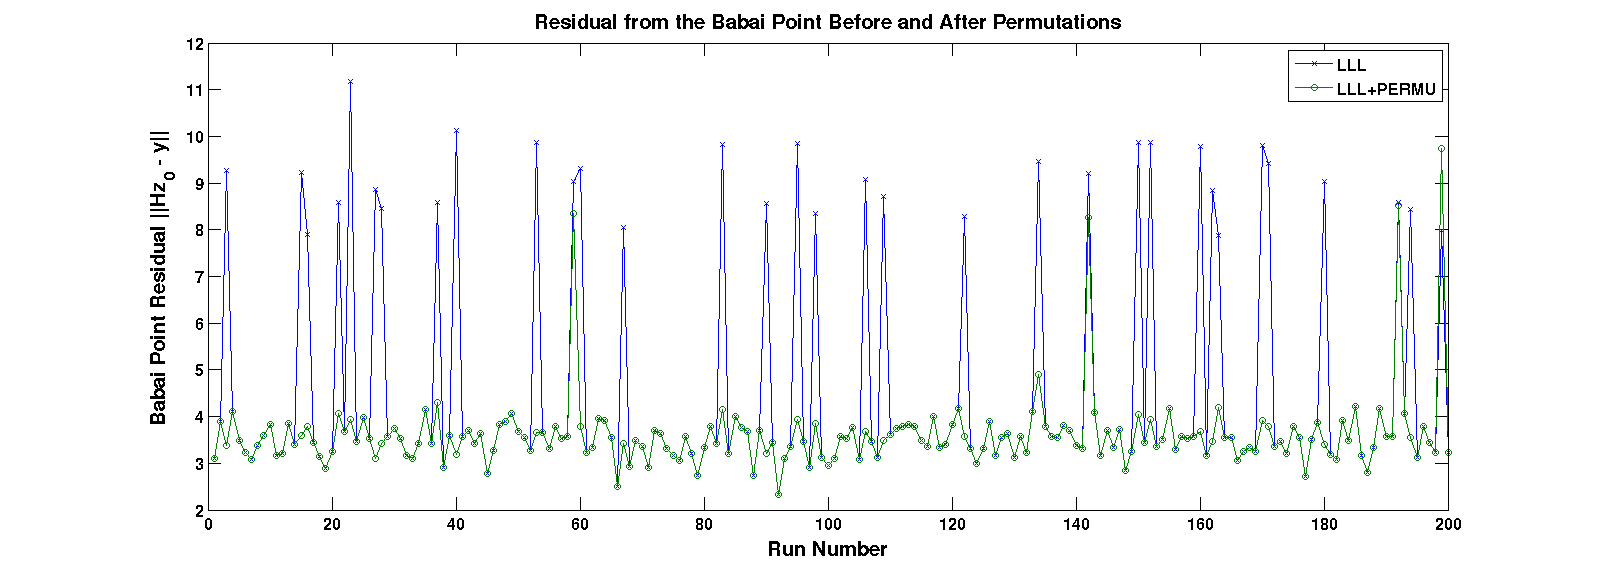
\includegraphics[width=6in,height=3in]{lllvslllpermubabai.png}
\caption{LLL Reduction vs LLL+PERMU. Residual from the Babai points.}
\label{fig:LLLvsPermuBabai}
\end{figure}

Looking at figure \ref{fig:LLLvsPermuBabai}, we can see that after permutations, the Babai point in this case is at least as good as the one before permutation. Often it is significantly better. For cases where the Babai point is better, we can choose to use the permuted $R$ for the search process. Numerical results comparing this strategy to performing the search on a LLL reduced matrix can be found in section \ref{sec:ILSReductionResults}.

Unforunately, there are certain special types of ill conditioned problems where the above strategy does not work very well. Even though the new matrix $R$ after permutations gives a better Babai point, the search process visits more nodes. Some characteristics and examples of such problems are given in section \ref{sec:ILSReductionResults}. In these cases, we may use the permutation strategy just to help set an initial search radius $\beta$ from chapter \ref{chap:SESearch}. Then we may perform the search on the LLL reduced matrix $R$.

Since we only apply orthogonal transformations to the matrix $R$ and vector $y$ with our permutation strategy, we can use the residual from the Babai point in the permuted problem directly in the problem before permutation. The equation $\left \| VRPz_0 - Vy \right \|_2^2 = \left \| RPz_0 - y \right \|$, where $V$ is a product of Givens rotations and $P$ is a permutation matrix, shows this. This means the $\beta$ given by this strategy will never be too small, forcing us to restart the search process. Using this residual in the search process on the LLL reduced problem when it is smaller than the residual to the Babai point given by LLL reduction alone is guaranteed to result in a faster search time. From here on we will refer to this strategy as LLL+BABAI. Since the permutation reduction process is very fast compared to the search, usually the overall run time, which is the time for the search plus the time for reduction, will be faster as well. There are some cases where we obtain better results by using the permuted matrix $R$ in the search, but as a general method to solve ILS problems, it is safer to use the LLL reduced $R$ with the initial radius $\beta$ given by the permutation strategy. Some comparisons can be found in section \ref{sec:ILSReductionResults}.

\vsp \subsection{ILS Reduction Results} \label{sec:ILSReductionResults}
In this subsection, some results will be presented to compare the speed of the search process after applying the reduction strategies presented previously in this chapter. We will compare the LLL reduction, LLL reduction plus permutations (LLL+PERMU), and the LLL reduction using the initial radius $\beta$ given by the permutation strategy (LLL+BABAI).

Figure \ref{fig:LLLvsPermuvsBabai} shows the three reduction strategies compared when run on normally distributed, random matrices $H$ of sizes from $35 \times 35$ to $50 \times 50$. The horizontal axis displays varying values for $\sigma$ which is the noise parameter. The vertical axis is the average time taken for the search process over $200$ runs where on each run a new matrix $H$, vector $x$ and noise vector $v$ were generated.

\begin{figure}
\centering
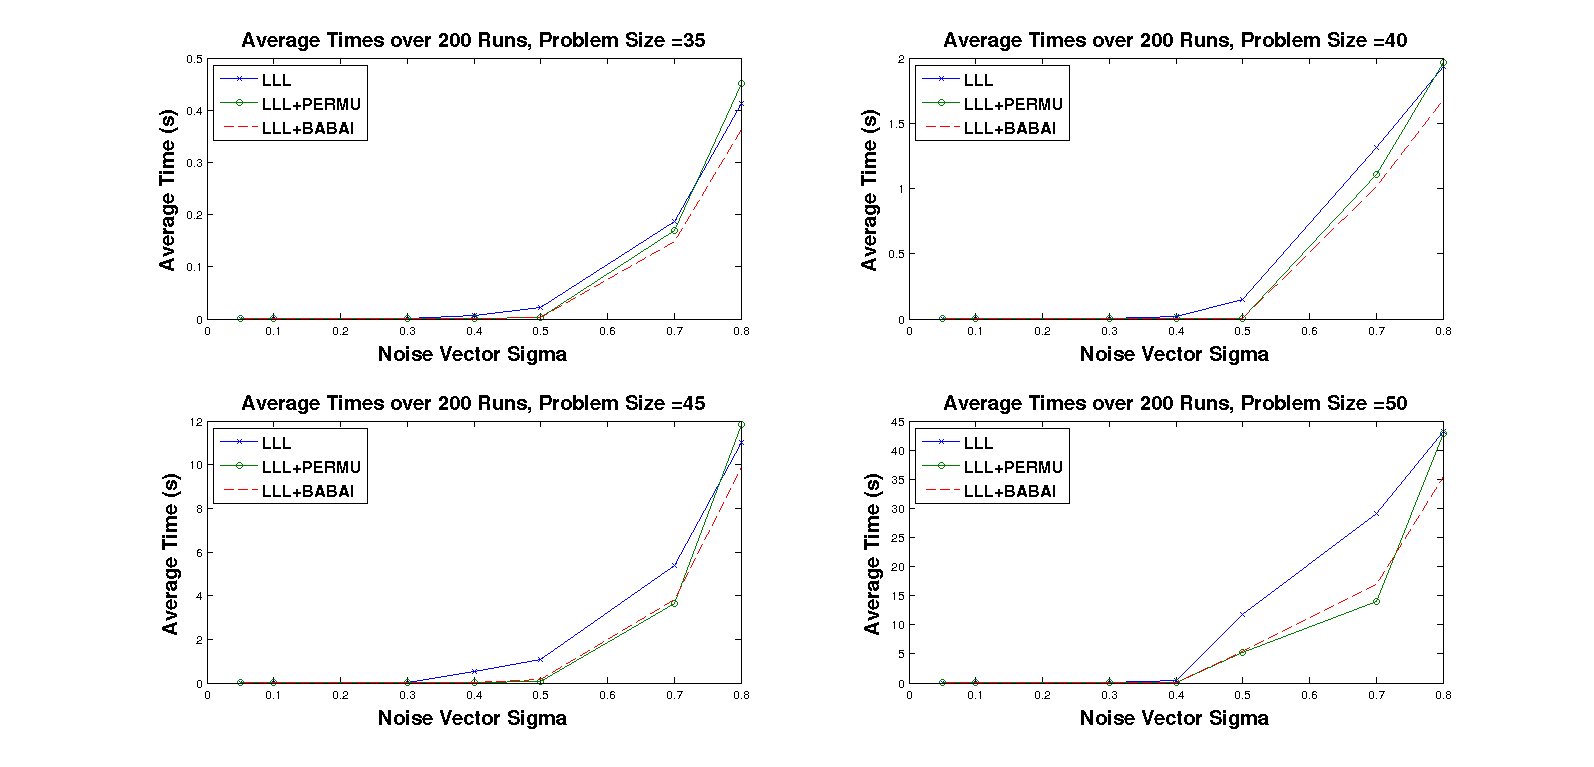
\includegraphics[width=6.5in,height=5in]{lllvspermuvsbabai.png}
\caption{LLL Reduction vs LLL Reduction and Permutations vs LLL Reduction with Permutation Initial Radius.}
\label{fig:LLLvsPermuvsBabai}
\end{figure}

Looking at figure \ref{fig:LLLvsPermuvsBabai}, we see that when the noise is small, the search process is too fast for any extra reduction to make a difference. As the noise becomes larger, LLL+PERMU starts to offer a significant advantage in terms of search time. LLL+PERMU and LLL+BABAI perform similarly at moderate levels of noise in this case. As the noise rises further, LLL+PERMU actually becomes worse than LLL, however LLL+BABAI maintains a significant advantage in all cases.

\begin{table} \label{tab:successRateLLL}
\caption{Success Rate (out of 200) for LLL Reduction on various problem sizes and levels of noise.}
\begin{tabular}{|l|l|l|l|l|l|l|l|} 
\hline
 &              $0.05$ & $0.1$ & $0.3$ & $0.4$ & $0.5$ & $0.7$ & $0.8$ \\ \hline
$35 \times 35$& $200$  & $200$ & $199$ & $192$ & $178$ & $89$  & $44$\\ \hline
$40 \times 40$& $200$  & $200$ & $200$ & $196$ & $175$ & $75$  & $45$\\ \hline
$45 \times 45$& $200$  & $200$ & $200$ & $193$ & $175$ & $79$  & $42$\\ \hline
$50 \times 50$& $200$  & $200$ & $200$ & $196$ & $167$ & $89$  & $44$\\
\hline
\end{tabular}
\end{table}


\begin{table} \label{tab:successRatePermu}
\caption{Success Rate (out of 200) for LLL+PERMU on various problem sizes and levels of noise.}
\begin{tabular}{|l|l|l|l|l|l|l|l|} 
\hline
 &              $0.05$ & $0.1$ & $0.3$ & $0.4$ & $0.5$ & $0.7$ & $0.8$ \\ \hline
$35 \times 35$& $200$  & $200$ & $200$ & $200$ & $198$ & $132$  & $76$\\ \hline
$40 \times 40$& $200$  & $200$ & $200$ & $200$ & $198$ & $120$  & $77$\\ \hline
$45 \times 45$& $200$  & $200$ & $200$ & $200$ & $194$ & $141$  & $86$\\ \hline
$50 \times 50$& $200$  & $200$ & $200$ & $199$ & $196$ & $137$  & $94$\\
\hline
\end{tabular}
\end{table}

Tables \ref{tab:successRateLLL} and \ref{tab:successRatePermu} show how many times out of $200$ runs that the Babai point was equal to the true solution $x$. If we take this as a percentage it is known as the "Success Rate". This is an important number because many practical applications may decide not to solve the ILS problem completely and instead just use the Babai point as an estimate at the solution. Here we see that the LLL+PERMU strategy can offer a significantly better success rate in all cases tested; even in cases where the search process may be slower on average if we use the permuted $R$.

It is not fully clear why LLL+PERMU fails to perform well in the search process when the noise is high. One reason is because the matrix $R$ after the permutations is usually further from a LLL reduced matrix when the noise is high as opposed to when the noise is low. This has been confirmed through numerical experiments where when the second inequality in \ref{eq:LLLConditions} was not satisfied, the difference $r_{k-1,k-1}^2 - (r{k,k}^2 + r{k-1,k}^2)$ was added to a sum. For a LLL reduced matrix this sum taken from $1 \dots n$ should be $0$, as the matrix becomes further from LLL reduced the sum will increase. A rough explanation as to why this happens is as follows; when the noise is very low the permutation algorithm finds the column permutations that maximize the diagonal entries in the order from $n \dots 1$. As the noise rises, this property is lost. To see this consider the motivation for the CH algorithm in \ref{subsec:CH} and consider what happens when $y = Hx$. One goal of the LLL reduction is also to maximize the diagonal entries in order from $n \dots 1$ in a way, it however also considers the off diagonal and previous diagonal entry. When the noise is lower, the permutation algorithm is likely to do fewer permutations since the ordering is more likely to already be somewhat satisfied since we started with a LLL reduced matrix. Therefore the matrix is likely to remain closer to a LLL reduced matrix.

The next set of results demonstrates a case where the permutation strategy should not be used. In figures \ref{fig:lllvspermubabaiill} and \ref{lllvspermuill} the matrix $H$ is generated by first generating two random, normally distributed matrices $A$ and $B$. Then the $QR$ factorization of each matrix is taken, so we will have $A = Q_AR_A$ and $B = Q_BR_B$. Next we generate a diagonal matrix $D$, where $d_{ii} = 10^{-\frac{(i-1)*4}{(n-1)}}$. Recalling that the condition number of a matrix is the first singular value divided by the last one; we will construct a  matrix with condition number $10^4$ by forming the product of the SVD, $H = Q_ADQ_B$. We generate $x$ and $y$ in the same way as the previous results.

\begin{figure}
\centering
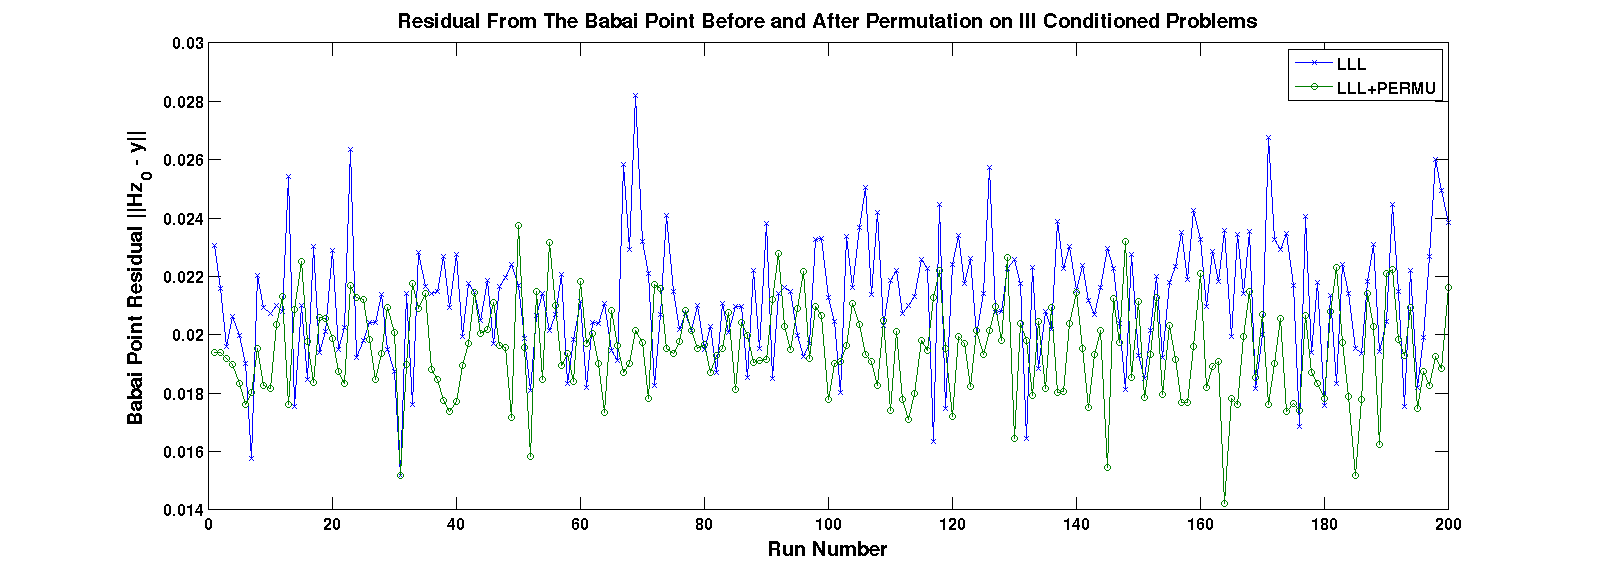
\includegraphics[width=6in,height=3in]{lllvspermubabaiill.png}
\caption{LLL Reduction vs LLL + PERMU. Residual from the Babai points on ill conditioned problems.}
\label{fig:lllvspermubabaiill}
\end{figure}

\begin{figure}
\centering
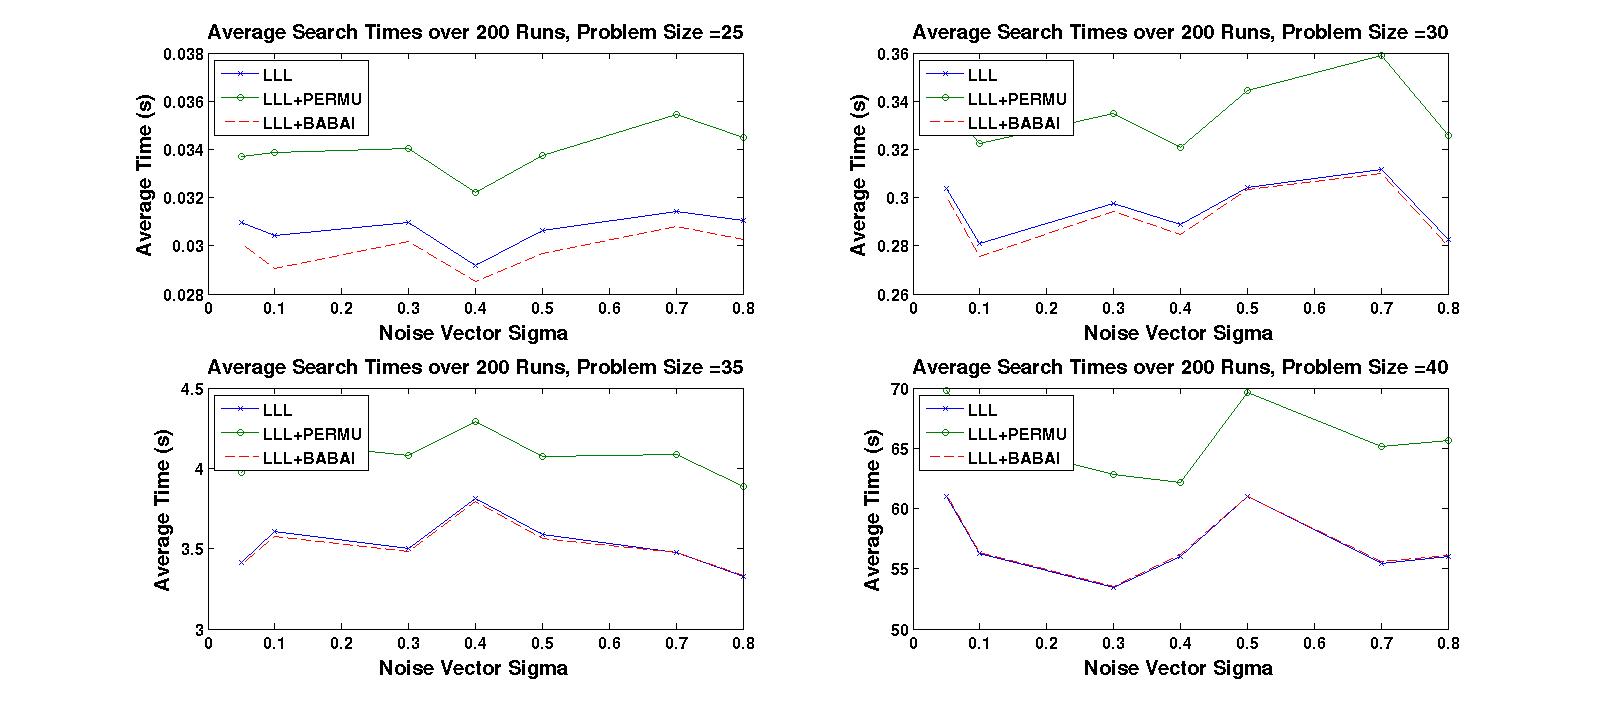
\includegraphics[width=6.5in,height=5in]{lllvspermuvsbabaiill.png}
\caption{LLL Reduction vs LLL +PERMU vs LLL + BABAI on ill conditioned problems.}
\label{fig:lllvspermuvsbabaiill}
\end{figure}

Figure \ref{fig:lllvspermubabaiill} shows the residual for the Babai point both before and after permutation where $H \in \mathbb{R}^{40 \times 40}$ and $\sigma = 0.5$. Comparing to figure \ref{fig:LLLvsPermuBabai}, we notice that it is much different. First, the residual both before and after permutation is much smaller in magnitude. The residual after permutation is slightly better than before on average, but the difference is nearly insignificant. With the smaller residual one may expect that the Babai point in this case is more likely to be equal to the true solution $x$. This however is not the case at all. Out of the $200$ runs in figure \ref{fig:lllvspermubabaiill}, not once was the Babai point equal to the true solution; compared to the example in figure \ref{fig:LLLvsPermuBabai} where $167/200$ times the Babai point was the correct solution before permutations were performed.

Knowing that the Babai point does not seem to be significantly better when the matrix $H$ is generated in this way, we can predict that the run time performance of the search process will probably be worse in the case where we use LLL+PERMU and about the same for LLL+BABAI. Figure \ref{fig:lllvspermuvsbabaiill} confirms this.

\chapter{Alternate Search Strategies} \label{chap:Searches}

Chapter \ref{chap:SESearch} described the most common search strategy used to solve both the ILS and BILS problems. Also, the search process was shown to be equivalent to a tree search problem where we must find the minimum cost leaf in a tree of height $n$ with potentially exponential width. The difference between this tree search and more general tree search problems is that we can easily visit the children of a given node in increasing order of cost (partial residual); we can compute the next child to visit in constant time. 

While the depth first search corresponding to the SE algorithm is usually very fast, it is not optimal in terms of the number of nodes visited during the search process. Let $x_{i:n}^p$ denote the node in the search tree that results from fixing $x_{i:n}$ to some particular set of values, we may call this a partial solution. Then the partial residual given by this partial solution is equivalent to its cost in the search tree and can be defined as $\left \| R_{i:n,i:n}x_{i:n}^p - \bar{y}_{i:n}\right \|_2^2$. An optimal algorithm for the ILS problem visits only nodes in the search tree with partial residuals that are less than the optimal ILS solutions residual. Therefore all nodes explored by the optimal search process will satisfy the following:
\begin{equation}\label{eq:optimalSearchCond}
\left \| R_{i:n,i:n}x_{i:n}^p - \bar{y}_{i:n}\right \|_2^2 \le \left \| Rx_{ILS} - \bar{y} \right \|_2^2
\end{equation}

Where $x_{ILS}$ here denotes the optimal ILS solution, which depending on the noise may not be the same as the original integer vector. Assuming no other special knowledge of the search problem, any other search algorithm must at least explore this set of nodes to guarantee there is no other leaf in the tree with a lower residual than the one found. There are in fact ways to reduce the number of nodes visited beyond this point, one technique involves using lower bounds on the optimal solutions residual. Unfortunately after numerical testing it was found that these methods incur too much per-node overhead to provide faster solutions to {\em reduced} ILS and BILS problems.

One algorithm that satisfies the requirement in \eqref{eq:optimalSearchCond} is called the "Best First Search" which will be referred to as BFS from here on for convienience. This algorithm has been proposed in the literature a number of times, \cite{FukMU04} and \cite{XuWZW04} are two examples, although they appear different on the surface. Later in this chapter a detailed description of the BFS will be given. For now it is enough to note that the BFS pays a price to achieve the goal of expanding the minimum number of nodes, it must permanently store each node explored during the search in memory and always keep track of the node with minimum cost. Also, when the nodes are later accessed from memory, since they are not stored in a simple manner like the SE search, it is likely that we will incur cache penalties when accessing nodes. For these reasons it is not always practical to use the BFS strategy, one problem is that often hardware applications have limited memory, another is that when the number of nodes explored becomes very large, the overhead of finding the one with minimum cost becomes significant and this must be done at each iteration.

Unfortunately, some of the literature such as \cite{StuBF07} does not properly consider the overhead of finding the minimum cost node when comparing search algorithms, instead only considering the goal of limiting the memory usage of BFS while still exploring as few nodes as possible. Comparing the number of nodes explored by two different search processes may not always be meaningful if one process spends much more time on each node than the other.

The following sections will explain the BFS, quickly overview a couple of attempts that have been made to control the memory usage of the BFS, and then propose a new idea for combining the BFS with the SE search in order to limit memory usage and decrease computational complexity.

\vsp \section{Best First Search} \label{sec:BFS}

A quick review from chapter \ref{chap:SESearch}; we will explore the search tree which has depth $n$ and each edge has a cost to traverse. Define a given nodes cost as the sum of the costs of all the edges traversed to reach the node, that is the length of the path between the node and the root. This cost is equal to the partial residual for fixing $x_{i:n}$ to a set of values, e.g. $\left \| R_{i:n,i:n}x_{i:n}^p - \bar{y}_{i:n}\right \|_2^2$. We would like to find the leaf with minimal cost. For the BFS, we will define a nodes ``next best child" as the child of that node with the lowest cost that has not yet been visited. This is simple to compute; the first ``next best child'' for a node is just $\lfloor c_k \rceil$ as defined in chapter \ref{chap:SESearch}. The next will be $\lfloor c_k \rceil \pm 1$, such that we get the second nearest integer to $c_k$, we proceed in this way, always taking the next nearest integer to define the ``next best child''. This is the exact same strategy that the SE search uses.

The core data structure used to efficiently implement a best first search is called a priority queue. The priority queue is an abstract data structure whose basic operations are $insert(element,cost)$, and $findmin()$. The $insert(element,cost)$ operation adds an element to the queue with some real value cost. The $findmin()$ operation finds and removes the element with minimum cost from the queue. The implementation details are not particularly relevant to this thesis, but it is important to note that there are various implementations used in practice. The usual cost for the $insert(element,cost)$ operation is $\theta(1)$ and for the $findmin()$ operation $\theta(log(N))$ where $N$ is the number of elements currently in the queue.

As mentioned above, for the ILS application, we can quickly find a given nodes ``next best child", it is the node corresponding to the next choice of $x_k$ chosen as in the SE algorithm. The ``first best child'' of a node at level $k-1$ assuming $x_{k-1:n}$ are fixed, is always the node corresponding to $x_k = \lfloor c_k \rceil$, where $c_k$ comes from \eqref{eq:searchC}.

In the first step of the BFS, we initialize an empty priority queue, $pq$ and define the root node as having a cost of $0$ and being at level $n+1$. The ``next best child" of the root node will correspond to $x_n = \lfloor \bar{y}_n/R_{n,n} \rceil$ and the cost to visit this child will be equal to the partial residual $(R_{n,n}x_n - \bar{y}_n)^2$, we will call this cost the ``next best child cost". The root node will store its current ``next best child" and ``next best child cost" and then be inserted into $pq$, elements in this priority queue will always be sorted by their ``next best child cost".

In the next step, we will visit the first child of the root, $x_{n-1}$. First, we perform the $findmin()$ operation on the priority queue, since currently the root is the only element, it will be returned. We would like to visit the first child of the current node (which is now the root). To visit a node involves calculating the ``next best child" and the ``next best child cost", therefore we must compute these quantities for the node corresponding to $x_{n}$ (which is the first child of the root). The ``next best child" of $x_n$ will be given by $x_{n-1} = \lfloor c_{n-1} \rceil$ and its cost  will be the partial residual $\left \| R_{n-1:n,n-1:n}x_{n-1:n}^p - \bar{y}_{n-1:n}\right \|_2^2$. We then insert $x_n$ into the priority queue with its ``next child'' and ``next child cost''. Notice if we expand the cost as follows, $(R_{n,n}x_n - \bar{y}_n)^2 + (R_{n-1,n}x_n + R_{n-1,n-1}x_{n-1} - \bar{y}_{n-1})^2$ that the first term in the cost is just the cost of the parent node; this means to calculate the cost for a child at level $i$, we only need to add the $i^{th}$ term from the sum defined by $\left \| R_{i,i:n}x_{i:n}^p - \bar{y}_{i}\right \|_2^2$ to the cost of the parent.

Since we are now visiting the first child of the root, we must generate the roots new ``next best child", $x_n = \lfloor c_n \rceil ^+_- 1$ and the cost for this child (also the partial residual), $(R_{n,n}x_n - y_n)^2$. We may now insert the root back into the priority queue with the newly calculated ``next best child cost" and ``next best child''.
 
At this step, the next node to be visited will be the one at the top of the priority queue with the smallest ``next best child cost". Currently there are two nodes in the priority queue, one at level $n$ and one at level $n-1$. If the former is smaller, we will visit the second best child of $x_n$, the new $x_{n-1}$ next, otherwise we will visit the best child of the node $x_{n-1}$ which is in the queue.

By proceeding in this way, we always visit the nodes in the order of increasing partial residual. The next node we visit is always the one with the next smallest partial residual (in the whole tree) from the previous one, even if those 2 nodes are at different levels. In this way we can guarantee that the first time we find a leaf in the tree, it must be the leaf with the smallest squared residual and is therefore the solution. Also, at the point where we find a leaf, we know we have explored only and all of those nodes that have a partial residual within the radius of the optimal hyper-sphere.

It should also be noted that trivial modifications to this BFS search algorithm can be made so that it will solve the BILS problem. We just need to make sure that at every step, the value chosen for $x_k$ is within the proper bounds defined in \ref{eq:boxCon}.

\vsp \section{Controlling BFS Memory Usage}

In \ref{sec:BFS}, notice that in each step a new node is added to the priority queue, but nodes are never removed (yes, the $findmin()$ operation removes a node, but we just update the cost and insert it back in). This means that each node visited during the search will be kept permanently in the priority queue. Since the number of nodes visited can potentially be exponential in $n$ this can become a problem for two reasons. The first and most obvious reason is memory usage. The second which is often over looked is, as the priority queue grows, it costs more and more to maintain it at each step; the cost for each operation is $\theta(log(N))$, where $N$ is the number of nodes visited so far. Depending on the implementation of the priority queue, there could also be some significant constants involved with this cost meaning that for even small $N$ we are paying a significant overhead to maintain the priority queue. Also consider that the cost to visit a node in an efficient implementation of the SE algorithm is only about $2k$, where $k$ is the level of the node in the tree.

With the rough cost analysis in the previous paragraph, it should be obvious that just because the BFS will explore fewer nodes than SE, does not mean it will be faster. In both \cite{DaiY08} and \cite{StuBF07} the authors try to find a balance between the number of nodes that we keep in memory at any given time, and visiting the smallest number of nodes possible; this section will briefly describe the approach taken in \cite{StuBF07}. Note that the algorithm described here is slightly different in that an extra parameter has been eliminated, according to the authors results, this parameter seems to always make the performance worse anyways. It is not clear why they included it in their paper and it would just take longer to explain.

The idea is only slightly different from the BFS. The authors do not use the concept of a priority queue, and instead use ordered lists to find the node with minimal cost at each step. Suppose we have a list $S$ in which nodes are stored, also this list is sorted by each nodes level in the search tree (lower levels are toward the back). This list, like the priority queue in the BFS starts with only the root node. At each step, a new node is added to the back of the list by finding the node with minimal cost in $S$ (this will take $|S|$ operations) and visiting its ``next best child''. Now suppose we allow the user to specify some parameter $\alpha$. Instead of scanning the whole list $S$ to find the node with the lowest ``next best child cost'' to visit next, we simply look at the last $\alpha$ elements in $S$ (which correspond to the $\alpha$ lowest nodes in the tree) and make our decision based on these. Such a strategy forces the BFS to proceed down the tree much faster than it would otherwise.

Unfortunately, when a leaf is reached, we no longer have the guarantee that it is the optimal solution. We do know however that we no longer have to consider any of the last $\alpha$ nodes in $S$ since they all must have a cost greater than the cost of the leaf we had just found. We may remove the last $\alpha$ nodes in $S$, update the search radius to be the residual given by this leaf, and continue the BFS. Any time a node is visited with a ``next best child cost'' that is greater than the current search radius, we may discard the last $\alpha$ nodes in $S$. When $S$ is empty we may terminate with the optimal solution.

The authors also give some good bounds on the amount of memory this algorithm requires based on how the parameter $\alpha$ is chosen. They present some results, but do not give FLOP counts or CPU time, instead focusing on memory usage and the number of nodes visited.

There are a few drawbacks to this algorithm. One is that it is not clear how to implement this in practice. Consider setting the parameter $\alpha$ to a relatively high number. When $\alpha$ is higher, we will explore fewer nodes since it will be closer to the BFS, and we will discard more nodes each time we have the opportunity to discard. Unfortunately as $\alpha$ gets larger, a naive list based implementation becomes impractical. Scanning through $\alpha$ elements in a list at each step could impose significant overhead. Also consider that $S$ must be sorted by the nodes levels in the search tree. If we wish to add a new node which has a level larger than the smallest leveled nodes currently in $S$, we must move all of the lower nodes in the tree one place to the right in memory, again this could cost $\alpha$ operations. This suggests that we may want to use a priority queue based implementation for large alpha and a list based implementation for small alpha. 

With these problems, it is worthwhile to explore some other options to limit the memory usage of the BFS, but at the same time also try to decrease the amount of time spent processing each node in the tree.

\vsp \section{Combining BFS and SE Search}

Here a new method for controlling the memory usage of the BFS will be presented. Like the method in \cite{StuBF07} it is quite simple and relies on a parameter supplied by the user.

One of the main problems with the SE search occurs when elements high up in the tree (e.g. $x_n, x_n-1 \dots$) are initially chosen incorrectly. We must explore the entire subtree looking for the ILS solution, visiting many nodes that may have partial residuals higher than the residual given by the ILS solution. Eventually we make our way back up the tree to correct the mistake. The BFS doesn't have this problem since it does not restrict itself to visiting only children of the current node.

In order to avoid making expensive mistakes at high levels, we may consider cutting the search tree at some level $\alpha$ which will be supplied by the user. We begin with a BFS, when the BFS reaches a node at level $k=\alpha$, it uses a SE search to find the optimal solution in that nodes subtree. Suppose a we are at some node in the BFS which is given by fixing $x_{k+1:n}$ to some particular values (so we are at level $k=\alpha$), then we will solve the subproblem  given by:

\begin{align} 
&\hat{y} = y(1:k) - R_{1:k,k+1:n}x_{k+1:n} \\
&\min_{x_{1:k} \in {\mathbb{Z} }}  \| \hat{y} - R_{1:k,1:k}x_{1:k} \|_2
\end{align}

By solving this subproblem, we can find the optimal solution assuming $x_{k+1:n}$ are fixed. With the solution calculated by the SE algorithm, we can continue the BFS until we reach another node at level $\alpha$. Next time we visit a node at level $\alpha$, we again perform an SE search to find the optimal solution in this nodes subtree, however this time we may use a sphere constraint to terminate the SE search early; if the previous SE search found a leaf with some residual $r$, then we can terminate this SE search when there are no nodes with residual less than $r$ remaining to visit, we need not find a leaf. Continuing this process, eventually we will reach a point where the next node to be visited in the BFS has a cost greater than the current sphere radius (given by the residual from the best leaf visited), at this point we may terminate with the optimal solution.

With this approach and an appropriate choice of the parameter $\alpha$, we can avoid making expensive mistakes at higher levels in the search tree. We also will incur a much smaller overhead to maintain the priority queue, since it will not contain nearly as many nodes if $\alpha$ is chosen to be near $n$, and with the smaller priority queue, there will be less memory usage. 

There are some useful tricks which can be used in conjunction with the combined search process to improve performance. Consider that the first SE search will very often be the one that costs the most in terms of run time. This is because we have no sphere constraint to use as a stopping condition and must solve the subproblem completely. The best case occurs when the first subproblem we solve contains the ILS solution, in this case we get the smallest possible sphere radius to use in subsequent SE searches as a stopping criteria, and will therefore prune more nodes. To make this more likely to occur, we may delay solving the first subproblem as follows. When we visit a node at level $\alpha$, we can decide not to solve the subproblem stemming from this node, instead we put the node into a list of ``unsolved subproblems'' and continue the BFS. One example of when we may not want to solve a subproblem is when the Babai point given by that subproblem has a large residual. Eventually we will need to perform the SE search to find a leaf, once a suitable node is visited by the BFS (one with a relatively low residual to the Babai point is a good choice), we perform the SE search and find a leaf in the tree corresponding to a potential solution. Now we simply go back to the list of ``unsolved subproblems'' and solve them all, using the residual from the previous solution as an initial sphere radius. The unsolved problems that had Babai points yielding high residuals are now likely to terminate much more quickly because not many nodes should be within the current sphere radius if the subproblem that we chose to solve gave a good solution. 

Finally, it should be mentioned that while this combined BFS and SE search strategy has been described in a way to solve ILS problems, it is also applicable to BILS problems. Only minor modifications must be made in order to ensure the elements of $x$ satisfy the constraints defined in \ref{eq:boxCon}.

\vsp \section{Search Strategy Results} \label{sub:SearchResults}
In this section, results will be given to compare the SE search, BFS and the combination of the two. To this point, there has not been much said about how to choose the parameter $\alpha$. This section will attempt to address this question through some numerical experiments. We need to choose $\alpha$ low enough to avoid mistakes at high levels in the tree, but high enough so that we get the advantages of the SE search being faster at processing each node. Note that when $\alpha = n$, we have a pure SE search, and when $\alpha = 1$, the combined search strategy degrades to a BFS. 

For all of the results in this section, the matrices will simply be generated randomly with elements drawn from a standard normal distribution. The vectors $x$ will have elements uniformly distributed between $-10 \dots 10$ and the vectors $y$ are generated as $y = Hx+v$ where $v$ is normally distributed with some standard deviation $\sigma$.

Figure \ref{fig:searchsurface} shows runtime results as the parameter $\alpha$ varies for $50$ different randomly generated problems of size $50 \times 50$. Here the noise vector was has $\sigma = 0.8$, which is quite high. The x-axis which varies from $1 \dots 50$ represents the choices of the parameter $\alpha$. The y-axis gives the search time in seconds, and each line down the z-axis represents one of the $50$ random problems. On the far right of the graph where $\alpha$ is small, we have a search process equivalent to the BFS and toward the left as $\alpha$ gets larger it is equivalent to the  SE search. Notice that on both ends there are sometimes spikes in the run time, while if we follow the line defined by $\alpha = x = 40$, we see that there is a consistent trough in the runtime. This is interesting and tells us that for this particular type of problem, it is best to choose the parameter $\alpha$ somewhere around $40$. Also notice that choosing the parameter slightly incorrectly is usually not a big deal, there is a fairly wide range of good choices. We know the search behaves fairly consistently as the parameter $\alpha$ changes, and there is a wide range for good choices of the parameter; to choose $\alpha$ for some new type of problem generated in some other way, it is recommended to simply run it a few times with various parameter settings and choose the one that performs best.

\begin{figure}
\centering
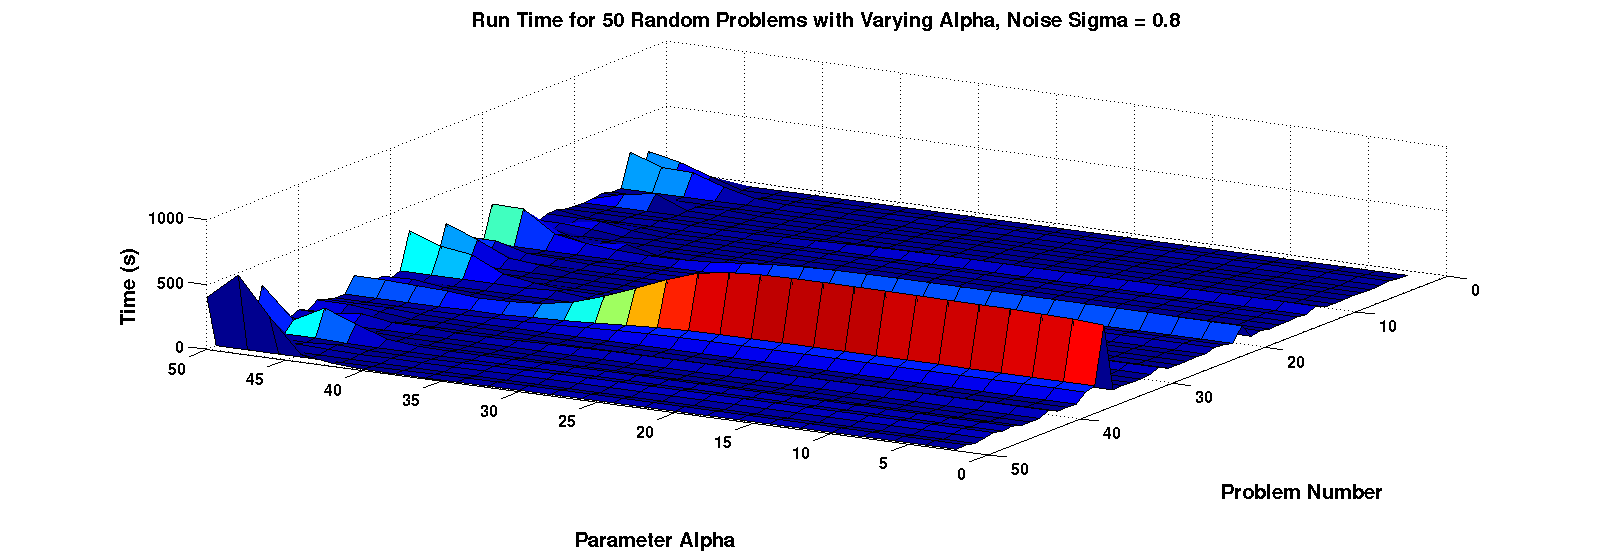
\includegraphics[width=6.5in,height=4in]{searchsurface.png}
\caption{Run time results for the combined search process with varying parameter $\alpha$.}
\label{fig:searchsurface}
\end{figure}

\chapter{Conclusions and Future Work} \label{chap:Conclusion}

This thesis focused on improving both the reduction and search processes in solving ILS and BILS problems. In chapter \ref{chap:Reduction} it was shown that two effective reduction strategies for the BILS problem are in fact theoretically equivalent. Using the knowledge of their equivalence a new reduction strategy was proposed that uses ideas from each to compute the same solution more efficiently and in a numerically stable manner. Also in Chapter \ref{chap:Reduction}, it was shown that under some practical conditions, this reduction process can be used to improve the performance of the ILS search process as well. This improvement seems to be a result of the Babai point after the permutations having both a lower residual and higher success rate (defined as the probability that the Babai point is equal to the true solution $x$). Since the Babai point has a tendency to have lower residual and higher success rate after applying these permutations, we can conclude that for both BILS and ILS problems, applications which use the Babai point as an estimate to the ILS solution should apply this permutations strategy in order to improve their success rate.

Some more investigation into the permutation reduction algorithm is still needed. It is not quite clear exactly when we should perform the search on the permuted matrix $R$ and when we should search the LLL reduced $R$. It is also possible that there exists another reduction strategy that can combine the properties of the permutations and LLL reduction. This was investigated but nothing significant was found. It would also be interesting if we could use some easy to calculate properties of the matrix $H$, vector $y$ and noise vector standard deviation $\sigma$ to decide whether we should use the permutations or not. Such a general result would be very useful in determining what types of practical applications this new reduction applies to.

In chapter \ref{chap:Searches} the ``Best First Search'' approach was described. The BFS has the property that it will visit the fewest nodes of any search algorithm. Unfortunately the BFS is not always ideal because of its high memory usage and complexity per node visited in the search tree. Previous attempts to improve upon the BFS were mentioned and a new one introduced. The new algorithm tries to address both the problem of memory usage and high complexity per node. Run time results were given comparing this new algorithm to the SE search process and the improvement was shown to be significant. 

It would be interesting to see if some theory could be worked out for how to choose the parameter $\alpha$ in the new search method. It is currently unclear how to choose it given a particular ILS problem. Since the optimal value for the parameter seems somewhat stable for fixed problem size and levels of noise, this may be possible.



\bibHeading{References}
\bibliography{../ILS}
\bibliographystyle{plain}

\index[abbr]{LS@LS: Least Squares}
\index[abbr]{ILS@ILS: Integer Least Squares}
\index[abbr]{BILS@BILS: Box-constrained Integer Least Squares}
\index[abbr]{SE@SE: Schnorr-Euchner enumeration algorithm}


\printindex[keylist]{Index}{Index}{}
\printindex[abbr]{KEY TO ABBREVIATIONS}{KEY TO ABBREVIATIONS}{}

\end{document}


 






